\documentclass[12pt,a4paper]{report}
\usepackage[top=2.5cm, bottom=2.5cm, left=2.5cm, right=2.5cm]{geometry}
\usepackage{amsmath}
\usepackage{amssymb}
\usepackage{graphicx}
\usepackage{tabularx}
\usepackage{algorithm}
\usepackage{algpseudocode}
\usepackage{listings}
\usepackage[usenames,dvipsnames,svgnames]{xcolor}
\usepackage{url}
\newcommand{\vect}[1]{\boldsymbol{#1}}
\usepackage{hyperref}
\hypersetup{
pdfnewwindow=true,      % links in new window
colorlinks=true,        % false: boxed links; true: colored links
linkcolor=Blue,         % color of internal links (change box color with linkbordercolor)
citecolor=Blue,         % color of links to bibliography
filecolor=Blue,         % color of file links
urlcolor=Blue           % color of external links
}


\begin{document}


\begin{center}
  \huge
  {
   \vspace*{1.0cm}
   GPUMD: \\
   Graphics Processing Units \\
   Molecular Dynamics\\
   \vspace*{1.0cm}
   Reference Manual\\
   \vspace*{1.0cm}
   Version 1.6\\
   \vspace*{1.0cm}
   (May 18, 2018)\\
  \vspace*{2.0cm}
  }
  \large
  {
  Authors: \\
  Zheyong Fan,
  Ville Vierimaa,
  Mikko Ervasti,
  Ari Harju \\
  Department of Applied Physics, Aalto University
  }
  \vspace*{1.0cm}
\end{center}


\tableofcontents


\chapter{Introduction}


\section{What is GPUMD?}

GPUMD stands for \textbf{G}raphics \textbf{P}rocessing \textbf{U}nits \textbf{M}olecular \textbf{D}ynamics. It is a new molecular dynamics (MD) code fully implemented on graphics processing units (GPUs). It was firstly used for heat transport simulations only but we are now making it more and more general.


\section{Citations}

If you use GPUMD in your published work, we kindly ask you to cite the following paper which describes the central algorithms used in GPUMD:

\begin{itemize}
\item Zheyong Fan, Wei Chen, Ville Vierimaa, and Ari Harju. Efficient molecular
dynamics simulations with many-body potentials on graphics processing units.
\textit{Computer Physics Communications}, 218:10-16, 2017.
\end{itemize}

If your work involves using heat current and virial stress formulas as implemented in GPUMD, the following paper can be cited:
\begin{itemize}
\item Zheyong Fan, Luiz Felipe C. Pereira, Hui-Qiong Wang, Jin-Cheng Zheng, Davide Donadio, and Ari Harju. Force and heat current formulas for many-body
potentials in molecular dynamics simulations with applications to thermal conductivity calculations. Phys. Rev. B, 92:094301, Sep 2015.
\end{itemize}

You can cite the following paper if you use GPUMD to study heat transport using the in-out decomposition for 2D materials and/or the spectral decomposition method as described in it:
\begin{itemize}
\item Zheyong Fan, Luiz Felipe C. Pereira, Petri Hirvonen, Mikko M. Ervasti, Ken R.
Elder, Davide Donadio, Tapio Ala-Nissila, and Ari Harju. Thermal conductivity
decomposition in two-dimensional materials: Application to graphene. Phys.
Rev. B, 95:144309, Apr 2017.
\end{itemize}

\section{Feedbacks}

You can e-mail the first author if you find errors in the manual or bugs in the source code, or have any suggestions/questions about the manual and code. The following email addresses can be used:
\begin{itemize}
\item zheyong.fan(at)aalto.fi (valid at least up to the end of 2019)
\item brucenju(at)gmail.com
\item zheyongfan(at)163.com
\end{itemize}


\section{Acknowledgments}
We acknowledge the computational resources provided by Aalto Science-IT project and Finland's IT Center for Science (CSC). We also thank the great help from the CUDA experts from NVIDIA and CSC during the GPU hackathon (13-09-2016 to 16-09-2016) organized by Sebastian von Alfthan.




\chapter{Features of GPUMD}


\section{GPU-accelerated force evaluation for many-body potentials}

One of the major features of GPUMD is that force evaluation for many-body potentials has been significantly accelerated by using GPUs. Our efficient and flexible GPU-implementation of the force evaluation for many-body potentials relies on a set of simple expressions for force, virial stress, and heat current derived in Ref. \cite{fan2015prb}. Detailed algorithms for the efficient CUDA-implementation have been presented in Ref. \cite{fan2017cpc}.

Using the methods as described in Refs. \cite{fan2015prb,fan2017cpc}, we have implemented various many-body potentials in GPUMD, including:
\begin{itemize}
\item The EAM-type potential with some analytical forms \cite{zhou2004prb,dai2006jpcm}.
\item The Tersoff (1989) potential with single or double atom types \cite{tersoff1989prb}.
\item The Stillinger-Weber (1985) potential \cite{stillinger1985prb}.
\item The Vashishta potential \cite{vashishta2007jap}.
\item The REBO potential for Mo-S systems \cite{liang2009prb}.
\end{itemize}
More many-body potentials will be implemented in GPUMD in future versions.

\section{Utilities for heat transport simulations}

Apart from being highly efficient, another unique feature of GPUMD is that it has useful utilities to study heat transport. The current version of GPUMD can calculate the following quantities related to heat transport:
\begin{itemize}
\item It can calculate the phonon density of states (DOS) from the velocity autocorrelation function (VAC), using the method of Dickey and Paskin \cite{dickey1969pr}.
\item It can calculate the equilibrium heat current auto-correlation (HAC), whose time integral gives the running thermal conductivity according to the Green-Kubo relation \cite{green1954jcp,kubo1957jpsj}. As stressed in Ref. \cite{fan2015prb}, the heat current as implemented in LAMMPS \cite{plimpton1995jcp} does not apply to many-body potentials and significantly underestimates the thermal conductivity in 2D materials described by many-body potentials. GPUMD also contains the thermal conductivity decomposition method as introduced in Ref. \cite{fan2017prb}, which is essential for 2D materials.
\item It can calculate the thermal conductivity of a system of finite length or the thermal boundary resistance (Kapitza resistance) of an interface or similar structures using non-equilibrium MD (NEMD) methods. The spectral decomposition method as described in Ref. \cite{fan2017prb} has also been implemented.
\end{itemize}



\section{Other features}

\subsection{Boundary conditions}

GPUMD supports the following boundary conditions in each direction:
  \begin{itemize}
  \item free boundary conditions
  \item periodic boundary conditions (using the minimum image convention)
  \item fixed boundary conditions (by fixing some atoms)
  \end{itemize}

The current version of GPUMD only supports orthogonal simulation boxes. Triclinic simulation boxes \textit{might} be implemented in a future version.




\subsection{Neighbor list construction}

GPUMD has the following two versions for neighbor list construction and automatically chooses an appropriate one according to the inputs:
  \begin{itemize}
  \item an $O(N^2)$ method which builds the Verlet neighbor list by directly checking the distance between one particle and all the other particles in the simulation box
  \item an $O(N)$ method which first builds a cell list and then converts the cell list to the Verlet neighbor list
  \end{itemize}
When the neighbor list is required to be updated during a simulation, one only has to specify a skin distance and the code will automatically determine when the neighbor list needs to be updated.

\subsection{Integration methods}

The velocity-Verlet \cite{swope1982jcp} integration scheme is used for all the ensembles.
The supported ensembles and the adopted methods are
  \begin{itemize}
  \item the $NVE$ ensemble
  \item the $NVT$ ensemble
    \begin{itemize}
    \item the Berendsen method  \cite{berendsen1984jcp}
    \item the Nos\'{e}-Hoover chain method \cite{nose1984jcp,hoover1985pra,martyna1992jcp,martyna1996mp,tuckerman2010}
        with a fixed chain length of 4.
    \end{itemize}
  \item the $NPT$ ensemble
    \begin{itemize}
    \item the Berendsen method  \cite{berendsen1984jcp} with the pressure in each direction controlled independently
    \end{itemize}
  \end{itemize}

We are working on implementing more integration methods.

\section{Major changes compared to the previous versions}

\subsection{Major changes introduced in version 1.1}
\begin{enumerate}
\item Added a potential model for single-layer black phosphorene as introduced by Xu \textit{et al.} \cite{xu2015jap}.
\end{enumerate}

\subsection{Major changes introduced in version 1.2}
\begin{enumerate}
\item In the previous versions, the initial velocities have zero linear momentum but generally nonzero angular momentum. This will not result in rotation of the system if periodic boundary conditions are applied in two or three directions, but will result in rotation in systems with only one or no periodic direction. In version 1.2, both linear and angular momenta of the initial velocities are zeroed.
\end{enumerate}

\subsection{Major changes introduced in version 1.3}
\begin{enumerate}
\item Added the REBO (reactive empirical bond-order) potential for Mo-S systems developed by Liang \textit{et al.} \cite{liang2009prb,liang2012prb_erratum}. Note that the Lennard-Jones part was not included. We plan to include the Lennard-Jones part in a future version of GPUMD. 
\end{enumerate}


\subsection{Major changes introduced in version 1.4}
\begin{enumerate}
\item Added the Vashishta potential \cite{vashishta2007jap}.
\end{enumerate}


\subsection{Major changes introduced in version 1.5}
\begin{enumerate}
\item Added the general two-element Stillinger-Weber potential. The potential for single-layer black phosphorene introduced in version 1.1 is of this type and is thus removed.
\end{enumerate}

\subsection{Major changes introduced in version 1.6}
\begin{enumerate}
\item Added the tabulated Vashishta potential, which is about two times as fast as the analytical version when the relative force error is about $10^{-6}$.
\item The performance of the many-body potentials has been enhanced by about 50\%.
\end{enumerate}




\section{TODO List}

Here I list a few features which I will hopefully implement this or the next year:
\begin{itemize}
\item More Tersoff-type potentials
\item Spline-based EAM potential
\item Mixed potentials
\item Machine-learning potentials
\item The NPT integrator based on the MTK equation
\item Multi-GPU version of GPUMD
\end{itemize}


\chapter{Theoretical formalisms and numerical algorithms}

\section{Physical units used in the program}

The basic units in the numerical calculations are chosen to be
\begin{enumerate}
\item Energy: eV (electron volt)
\item Length: \AA~(angstrom)
\item Mass: amu (atomic mass unit)
\item Temperature: K (kelvin)
\item Charge: e (elementary charge)
\end{enumerate}
The purpose of using these units is to make the values of most quantities in the code close to unity. The units for all the other quantities are thus fixed. Here are some examples:
\begin{enumerate}
\item Time: \AA~amu$^{1/2}$ eV$^{-1/2}$, which is about $1.018051 \times 10^{1}$ fs
\item Velocity: eV$^{1/2}$ amu$^{-1/2}$
\item Force: eV \AA$^{-1}$
\item Pressure (stress): eV \AA$^{-3}$, which is about $1.602177 \times 10^{2}$ GPa
\item Thermal conductivity: eV$^{3/2}$ amu$^{-1/2}$ \AA$^{2}$~K$^{-1}$
      which is about $1.573769 \times 10^{5}$ W m$^{-1}$ K$^{-1}$
\item Boltzmann's constant: $k_B \approx 8.617343 \times 10^{-5}$ eV K$^{-1}$
\item Electrostatic constant:
$k_C = \frac{1}{4\pi\epsilon_0} \approx 1.441959 \times 10^{1}$ eV \AA~e$^{-2}$
\end{enumerate}

\textbf{Important note:}
The input and output files do not necessarily adopt these units. For example, time step in the input file is in unit of fs, rather than \AA~amu$^{1/2}$ eV$^{-1/2}$. Details on the units adopted by the input and output files are presented in Chapter \ref{chapter:usage}.


\section{Overall structure of the program}

GPUMD is written using CUDA C/C++. The overall style is C, without using classes (except for some C-style structures), but we might switch to C++ style in the future. Except for data initialization and some calculations that are very cheap or inherently serial, all the other calculations are done on the GPU.

The current version of GPUMD has 61 source files. Except for a few files ( \verb"main.cu", \verb"mic.cu", \verb"mic_template.cu"), all the other files come in pairs (e.g., \verb"gpumd" below means \verb"gpumd.cu" and \verb"gpumd.h"). The logical dependence of the files can be summarized as follows:

\begin{itemize}
\item \verb"main.cu" is the entrance of the program and depends on \verb"gpumd"
\item \verb"gpumd" depends on
  \begin{itemize}
    \item \verb"initialize"
    \item \verb"finalize"
    \item \verb"run"
  \end{itemize}
\item \verb"run" depends on
      \begin{itemize}
      \item \verb"potential"
      \item \verb"velocity"
      \item \verb"parse"
      \item \verb"dump"
      \item \verb"hac"
      \item \verb"shc"
      \item \verb"vac"
      \item \verb"heat"
      \item \verb"integrate"
      \item \verb"neighbor"
      \item \verb"validate"
      \item \verb"force"
      \end{itemize}
  \item \verb"integrate" depends on \verb"force"
  \item \verb"validate" depends on \verb"force"
  \item \verb"neighbor" depends on
        \begin{itemize}
        \item \verb"neighbor_ON1"
        \item \verb"neighbor_ON2"
        \end{itemize}
  \item \verb"force" depends on
        \begin{itemize}
        \item \verb"lj1"
        \item \verb"ri"
        \item \verb"eam_zhou_2004"
        \item \verb"eam_dai_2006"
        \item \verb"sw_1985"
        \item \verb"sw_1985_2"
        \item \verb"vashishta"
        \item \verb"tersoff_1989_1"
        \item \verb"tersoff_1989_2"
        \item \verb"rebo_mos2"
        \end{itemize}
  \item The files \verb"mic.cu" and \verb"mic_template.cu" will be directly included into some other files.
\item All the files (except for \verb"main.cu", \verb"mic.cu", and \verb"mic_template.cu") depend on \verb"common"
\end{itemize}




\section{Neighbour list construction}


We use the Verlet neighbor list when evaluating the forces between particles. Two methods for constructing the Verlet neighbor list are implemented, one is an $O(N^2)$ method and the other is an $O(N)$ method.


\subsection{A simple quadratic-scaling method}

In the $O(N^2)$ method, the Verlet neighbor list is constructed by directly checking the distance between every pair of particles. Therefore, the computational effort scales as $N^2$, where $N$ is the number of particles. This method only requires a single CUDA kernel.
Algorithm \ref{algorithm:neighbour_ON2} presents a pseudo code for the CUDA kernel.

\begin{algorithm}[htb]
\caption{The $O(N^2)$ method of neighbour list construction }
\label{algorithm:neighbour_ON2}
\begin{algorithmic}[1]
\Require $b$ is the block index
\Require $t$ is the thread index
\Require $S_b$ is the block size
\Require $i=S_b\times b+t$ is the particle index
\Require $N$ is the number of particles
\Require $r_c^2$ is the square of the cutoff distance for building the neighbor list
\Require NN$_{i}$ is the number neighbors for particle $i$
\Require NL$_{ik}$ is the index of the $k$th neighbor of particle $i$
\Require $\vect{r}_{i}$ is the position vector of particle $i$
\State $k\leftarrow 0$
\If {$i<N$}
    \State load $\vect{r}_{i}$ from the global memory
    \For {$j$ = 0 to $N - 1$}
        \If {$j = i$}
            \State continue
        \EndIf
        \State load $\vect{r}_{j}$ from the global memory and calculate
               $\vect{r}_{ij} = \vect{r}_{j} - \vect{r}_{i}$
        \State apply the minimum image convention to $\vect{r}_{ij}$
        \If {$|\vect{r}_{ij}|^2 < r_c^2$}
            \State NL$_{ik}\leftarrow j$
            \State $k\leftarrow k+1$
        \EndIf
    \EndFor
    \State NN$_{i}\leftarrow k$
\EndIf
 \end{algorithmic}
\end{algorithm}

In this kernel, the block size is $S_b$ and the grid size is $\left \lceil {N/S_b} \right \rceil$. The \textbf{if} statement is used to avoid manipulating invalid memory.


\subsection{A linear-scaling method}


In this method, one partitions the system into cells and only searches for neighbors of a given particle in a small number of cells. In 3D, there are $3^3=27$ cells to be searched, which does not scale with $N$. The overall computational effort of this method scales as $27N_0N \sim N$, where $N_0$ is the average number of particles in one cell. Therefore, this is a linear-scaling, or $O(N)$ method.

When periodic boundary conditions are applied, the number of cells in each direction is determined as
\begin{equation}
N_{x} = \lfloor L_x / r_c \rfloor;
\end{equation}
\begin{equation}
N_{y} = \lfloor L_y / r_c \rfloor;
\end{equation}
\begin{equation}
N_{z} = \lfloor L_z / r_c \rfloor.
\end{equation}
Here, $L_x$, $L_y$, and $L_z$ are the box lengths.
If a direction has free boundary conditions, we set the number of cells in that direction to $1$. The total number of cells is thus $N_c = N_x N_y N_z$.

With the number of cells determined, we next determine the number of particles $C_n ~(n=0, 1, \cdots, N_c-1)$ in each cell. We need to use a CUDA kernel to do this. A pseudo code for the kernel is presented in Algorithm  \ref{algorithm:cell_counts}.


\begin{algorithm}[htbp]
\caption{Determine the number of particles in each cell}
\label{algorithm:cell_counts}
\begin{algorithmic}[1]
\Require $b$ is the block index
\Require $t$ is the thread index
\Require $S_b$ is the block size
\Require $i=S_b\times b+t$ is the particle index
\Require $N$ is the number of particles
\Require $C_n$ is the number of particles in cell $n$ and has been initialized to 0
\If {$i < N$}
	\State calculate cell index $n$ of particle $i$
	\State atomic operation: $C_n \leftarrow C_n +1$
\EndIf
 \end{algorithmic}
\end{algorithm}

Note that atomic operations (for integer data) are used to avoid write conflict. In the above kernel, we need to calculate the cell index of a given particle (with coordinate components $x$, $y$, and $z$). This is done by using a device function. The total cell index $n$ is calculated from three indices:
\begin{equation}
n_x = \lfloor x / r_c \rfloor;
\end{equation}
\begin{equation}
n_y = \lfloor y / r_c \rfloor;
\end{equation}
\begin{equation}
n_z = \lfloor z / r_c \rfloor;
\end{equation}
\begin{equation}
n = n_x + N_x n_y + N_x N_y n_z.
\end{equation}
The cell index in the $x$-direction is required to be no less then 0 and no larger than $N_x-1$. That is, when $n_x < 0$, we increase $n_x$ by $N_x$; when $n_x \geq N_x$, we decrease $n_x$ by $N_x$. The other directions have similar requirements.

We then calculate the prefix sum (exclusive scan) $S_n$ of $C_n$:
\begin{equation}
S_0 = 0;
\end{equation}
\begin{equation}
S_n = \sum_{m=0}^{n-1} C_m \quad (1 \leq n \leq N_c-1).
\end{equation}
For this, we use the \verb"thrust::exclusive_scan" function from the thrust library.

Now we can determine which particles are in which cells. We define a one-dimensional array $I$ of length $N$, with $I_{S_n}$ to $I_{S_n + C_n - 1}$ being the indices of the particles in cell $n$. This array is constructed by using a CUDA kernel and a corresponding pseudo code is presented in Algorithm \ref{algorithm:cell_contents}.

\begin{algorithm}[htbp]
\caption{Determine the array $I$  containing the particle indices in the order of increasing cell index}
\label{algorithm:cell_contents}
\begin{algorithmic}[1]
\Require $b$ is the block index
\Require $t$ is the thread index
\Require $S_b$ is the block size
\Require $i=S_b\times b+t$ is the particle index
\Require $N$ is the number of particles
\Require $C_n$ is the number of particles in cell $n$ and has been initialized to 0
\Require $S_n$ is the prefix sum of $C_n$ as defined in the text
\Require $I_{S_n}$ to $I_{S_n + C_n - 1}$ are indices of the particles in cell $n$
\If {$i < N$}
	\State calculate cell index $n$ of particle $i$
    \State $I_{S_n + C_n} \leftarrow i$
	\State atomic operation: $C_n \leftarrow C_n +1$
\EndIf
 \end{algorithmic}
\end{algorithm}

Up to now, the so-called cell list has been constructed. The remaining task is to convert the cell list to the Verlet neighbor list. This can be done by using a CUDA kernel similar to that for the $O(N^2)$ method. A pseudo code is presented in Algorithm \ref{algorithm:convert}.

\begin{algorithm}[htb]
\caption{Construct the Verlet neighbour list from the cell list}
\label{algorithm:convert}
\begin{algorithmic}[1]
\Require $b$ is the block index
\Require $t$ is the thread index
\Require $S_b$ is the block size
\Require $i=S_b\times b+t$ is the particle index
\Require $N$ is the number of particles
\Require $r_c^2$ is the square of the cutoff distance for building the neighbor list
\Require $C_n$ is the number of particles in cell $n$
\Require $S_n$ is the prefix sum of $C_n$ as defined in the text
\Require $I_{S_n}$ to $I_{S_n + C_n - 1}$ are the indices of the particle in cell $n$
\Require NN$_{i}$ is the number neighbors for particle $i$
\Require NL$_{ik}$ is the index of the $k$th neighbor of particle $i$
\Require $\vect{r}_{i}$ is the position vector of particle $i$
\State $k\leftarrow 0$
\If {$i<N$}
    \State load $\vect{r}_{i}$ from the global memory
    \State calculate cell index $n$ of particle $i$
    \For  {$m$ in all the neighbor cells of cell $n$ (including cell $n$)}
        \For {$l$ = 0 to $C_m-1$}
            \State $j \leftarrow I_{S_m + l} $
            \If {$j = i$}
                \State continue
            \EndIf
            \State load $\vect{r}_{j}$ from the global memory and calculate
               $\vect{r}_{ij} = \vect{r}_{j} - \vect{r}_{i}$
            \State apply the minimum image convention to $\vect{r}_{ij}$
            \If {$|\vect{r}_{ij}|^2 < r_c^2$}
                \State NL$_{ik}\leftarrow j$
                \State $k\leftarrow k+1$
            \EndIf
        \EndFor
        \State NN$_{i}\leftarrow k$
    \EndFor
\EndIf
 \end{algorithmic}
\end{algorithm}

We note that the computation time used for the construction of the cell list is negligible compared to that used for the construction of the Verlet neighbor list from the cell list. However, we have to do this conversion because our efficient force evaluation algorithm \cite{fan2017cpc} requires using the Verlet neighbor list rather than the cell list. Fortunately, the neighbor list usually only needs to be updated every tens of time steps with a typical skin distance (defined as the difference between the cutoff distance used for building the neighbor list and the cutoff distance used for force evaluation). In some simulations such as calculating the thermal conductivity of stable solids, the neighbor list even does not need to be updated during the simulation.

\subsection{How to choose between the two versions?}

The $O(N)$ version is faster than the $O(N^2)$ version in most cases. But sometimes we still use the $O(N^2)$ version. Here are the choices made in GPUMD:
\begin{itemize}
\item If the number of cells in any direction with periodic boundary conditions is less than 3, the $O(N)$ version is not applicable (as some neighbors will be counted twice) and the $O(N^2)$ version will be used. Therefore, if you hope to use the $O(N)$ version, you should make sure that the number of cells in any direction with periodic boundary conditions is no less than 3.
\item The $O(N^2)$ version is only faster when the number of cells is very small. Take a 3D system with periodic boundary conditions in each direction for example, when the number of cells in each direction is 3, the $O(N^2)$ version is definitely faster than the $O(N)$ version, but the $O(N)$ version is already faster when the number of cells in each direction is 4. After doing some tests, we have decided to use the $O(N)$ version whenever the total number of cells is larger than 50. This might not be always optimal but is not a bad choice.
\item The $O(N^2)$ version is deterministic, but the $O(N)$ version contains randomness, due to the use of atomic operations in the CUDA kernels. Using atomic operations, the order of the neighbor particles for a given particle can be different from run to run, which is not desirable for the purpose of debugging. In view of this, we have provided a compiling option (see Chapter \ref{chapter:usage} for details) to switch on the debugging mode, where the $O(N^2)$ version is always used.
\end{itemize}
In summary, GPUMD chooses an appropriate method for neighbor list construction automatically and no input is expected from the users.


\subsection{How often should the neighbor list be updated?}

The frequency of updating the neighbor list depends on the applications. If one simulates a stable solid system with the initial neighbor list containing all the neighbors that has possible interactions with a given particle during the whole simulation, the neighbor list does not need to be updated at all. In other cases, the neighbor list needs to be updated during the simulation. Usually, one can set an updating frequency such as 10, which means that the neighbor list will be updated every 10 integration steps. However, this can be either inefficient or unsafe. Another way is to determine at every integration step whether the neighbor list needs to be updated by checking how far each atom has moved since the last neighbor list updating. It can be argued that the neighbor list should be updated when the maximum traveling distance of the particles since the last updating exceeds half of the skin distance (set by the user). As this check takes negligible time, GPUMD uses this method to determine automatically when the neighbor list is to be updated and thus does not expect the users to specify an updating frequency.








\section{General formalisms for force evaluation and related calculations}

\subsection{General form of empirical potential functions}


In classical molecular dynamics, the total potential energy $U$ of a system can be written as the sum of site potentials $U_i$:
\begin{equation}
\label{equation:U}
U=\sum_{i=1}^N U_i.
\end{equation}
The site potential can have different forms in different potential models. Although there are numerous potential models proposed to date, they can be largely classified into two groups: two-body potentials and many-body potentials.

\subsection{Force}

For two-body potentials, the site potential $U_i$ can be expressed as
\begin{equation}
\label{equation:U_i}
U_i= \frac{1}{2} \sum_{j \neq i} U_{ij}(r_{ij}).
\end{equation}
Here, $r_{ij} = |\vect{r}_j - \vect{r}_i|$ is the distance between particles $i$ and $j$ and $U_{ij}(r_{ij})$ is the pair potential between them.
The total force acted on particle $i$ can be derived to be:
\begin{equation}
\vect{F}_{i} = -\nabla_i U = \sum_{j \neq i}
\frac{\partial U_{ij}(r_{ij})}{\partial r_{ij}}
\frac{\vect{r}_{ij} }{r_{ij}}.
\end{equation}
In this manual, we use the symbol $\vect{r}_{ij}$ to denote the position difference vector from particle $i$ to particle $j$:
\begin{equation}
\boxed{\vect{r}_{ij} \equiv \vect{r}_j - \vect{r}_i}.
\end{equation}
The reader should bear this in mind when comparing the formulas in this manual with those in the literature, because many authors have used the opposite sign convention. One can also write the total force on particle $i$ in the following form:
\begin{equation}
\vect{F}_{i} = \sum_{j \neq i} \vect{F}_{ij},
\end{equation}
where
\begin{equation}
\vect{F}_{ij} =
\frac{\partial U_{ij}(r_{ij})}{\partial r_{ij}}
\frac{\vect{r}_{ij} }{r_{ij}}
\end{equation}
is the pairwise force acting on particle $i$ by particle $j$. Newton's third law is apparently valid here, in the sense that
\begin{equation}
\vect{F}_{ij} = - \vect{F}_{ji}.
\end{equation}

In some many-body potentials such as the embedded-atom method potential \cite{daw1984prb}, the site potential can not be written in the form of Eq. (\ref{equation:U_i}). In some other many-body potentials such as the Tersoff potential, the site potential can be written in the form of Eq. (\ref{equation:U_i}), but the $U_{ij}$ in this equation does not only depend on the distance between particles $i$ and $j$. The force formulas for many-body potentials have confused the community a lot. Recently, a well-defined force expression for general many-body potentials that explicitly respects Newton's third law  has been derived as \cite{fan2015prb}:
\begin{equation}
\vect{F}_{i} = \sum_{j \neq i} \vect{F}_{ij},
\end{equation}
where
\begin{equation}
\boxed{
\vect{F}_{ij} = - \vect{F}_{ji} =
\frac{\partial U_{i}}{\partial \vect{r}_{ij}} -
\frac{\partial U_{j}}{\partial \vect{r}_{ji}} =
\frac{\partial \left(U_{i} + U_{j}\right) }{\partial \vect{r}_{ij}}
}.
\end{equation}
Here, $\partial U_{i}/\partial \vect{r}_{ij}$ is a shorthand notation for a vector with cartesian components $\partial U_{i}/\partial x_{ij}$, $\partial U_{i}/\partial y_{ij}$, and $\partial U_{i}/\partial z_{ij}$. This pairwise force expression for many-body potentials has been confirm by Hardy \cite{hardy2016jcp} as well as by Chen and Diaz \cite{chen2016pre}. We have also confirmed its correctness by comparing with finite-difference calculations. This simple pairwise force expression for many-body potentials is the key for deriving well-defined expressions for other useful quantities such as virial stress and heat current, as discussed below.




\subsection{Stress}


Stress (tensor) is an important quantity in MD simulations. It consists of two parts: a virial part which is related to the force and an ideal-gas part which is related to the temperature. The virial part must be calculated along with force evaluation.

The validity of Newton's third law is crucial in simplifying the calculation of the virial stress. We know that the virial stress tensor is defined as
\begin{equation}
\textbf{W} = \sum_i \textbf{W}_i,
\end{equation}
\begin{equation}
\textbf{W}_i =
\vect{r}_{i} \otimes \vect{F}_{i}.
\end{equation}
Here, $\textbf{W}_i$ can be regarded as the per-atom virial stress. For periodic systems, the presence of absolute positions $\vect{r}_i$ would cause problems. However, when Newton's third law is valid, one can rewrite the per-atom virial stress as
\begin{equation}
\boxed{
\textbf{W}_i = -\frac{1}{2} \sum_{j \neq i} \vect{r}_{ij} \otimes \vect{F}_{ij}
},
\end{equation}
where only relative positions $\vect{r}_{ij}$ are involved. Because Newton's third law also applies to many-body potentials, the above expression of virial stress is valid for any classical potential.

The ideal-gas part of the stress is isotropic, which is given by the ideal-gas pressure:
\begin{equation}
p_{\text{ideal}}=\frac{Nk_BT}{V},
\end{equation}
where $N$ is the number of particles, $k_B$ is Boltzmann's constant, $T$ is the absolute temperature, and $V$ is the volume of the system.

Combining the ideal-gas part and the virial part, the total stress tensor $\sigma^{\alpha \beta}$ can be expressed as:
\begin{equation}
\sigma^{\alpha \beta} = -\frac{1}{2V} \sum_i \sum_{j \neq i}
r^{\alpha}_{ij} F^{\beta}_{ij} + \frac{Nk_BT}{V} \delta^{\alpha\beta}.
\end{equation}
Here, $\alpha$ and $\beta$ can be $x$, $y$, and $z$ and $\delta^{\alpha\beta}$ is the Kronecker symbol. We will denote the diagonal part of the total stress tensor as a ``vector'' $\vect{p}$ with components $p_x=\sigma^{xx}$, $p_y=\sigma^{yy}$, and $p_z=\sigma^{zz}$.
If the system is isotropic, we usually average the diagonal terms to get a scalar:
\begin{equation}
p = \frac{1}{3} \left(p_{x} + p_{y} + p_{z}\right) =
-\frac{1}{6V} \sum_i \sum_{j \neq i} \vect{r}_{ij} \cdot \vect{F}_{ij}
+ \frac{Nk_BT}{V}.
\end{equation}


\subsection{Heat current}


GPUMD can be used to compute the lattice thermal conductivity using the Green-Kubo \cite{green1954jcp,kubo1957jpsj} formula, which requires calculating the heat current.

In classical physics, the total heat current vector $\vect{J}$ of a system is defined to be\footnote{Actually, it is $J/V$ that has the dimension of heat current density (also called heat flux), which has the unit of W m$^{-2}$ in the international unit system. However, it is tedious to add the factor of $1/V$ in many of the subsequent equations.} the time derivative of the sum of the energy moments:
\begin{equation}
\vect{J} = \frac{d}{dt} \sum_i \vect{r}_i E_i.
\end{equation}
Here, $E_i$ is the site energy of particle $i$, which is the sum of the kinetic and potential energies:
\begin{equation}
E_i = \frac{1}{2}m_i \vect{v}_i^2 + U_i.
\end{equation}
Using Lebniz's rule, we have
\begin{equation}
\vect{J} = \sum_i \vect{v}_i E_i +  \sum_i \vect{r}_i \frac{d}{dt} E_i.
\end{equation}
The first term on the right hand side is usually called the convective term and we do not need to evaluate it in the force-evaluation kernel. The second term,
\begin{equation}
\vect{J}^{\text{pot}} = \sum_i \vect{r}_i \frac{d E_i} {dt},
\end{equation}
is usually called the potential term and needs to be evaluated in the force-evaluation kernel.

When using the Green-Kubo method, we need to use periodic boundary conditions (at least in the transport directions). For two-body potentials, we can arrive at the following expression which is suitable for implementation:
\begin{equation}
\vect{J}^{\text{pot}} = -\frac{1}{2} \sum_i \sum_{j \neq i}
\vect{r}_{ij}  \left( \vect{F}_{ij} \cdot \vect{v}_i \right).
\end{equation}
This equation can be expressed in an equivalent way:
\begin{equation}
\vect{J}^{\text{pot}} = -\frac{1}{2} \sum_i \sum_{j \neq i}
\left( \vect{r}_{ij} \otimes  \vect{F}_{ij} \right) \cdot \vect{v}_i .
\end{equation}
Therefore, we can also write it in terms of the per-atom virial:
\begin{equation}
\vect{J}^{\text{pot}} = \sum_i \textbf{W}_i \cdot \vect{v}_i.
\end{equation}
We can also define the per-atom heat current $\vect{J}_i^{\text{pot}}$ for the potential part in the following way:
\begin{equation}
\vect{J}^{\text{pot}} = \sum_i \vect{J}^{\text{pot}}_i;
\end{equation}
\begin{equation}
\vect{J}^{\text{pot}}_i = \textbf{W}_i \cdot \vect{v}_i.
\end{equation}

However, we note that the above formula only applies to two-body potentials. For many-body potentials, it has been demonstrated \cite{fan2015prb} that the above virial-based formula is wrong and the correct one is
\begin{equation}
\boxed{
\vect{J}^{\text{pot}}_i = \sum_{j \neq i} \vect{r}_{ij}
 \left(
 \frac{ \partial U_j} {\partial \vect{r}_{ji}} \cdot \vect{v}_i
 \right)}.
\end{equation}



The above heat current formula is usually applied in equilibrium simulations. In nonequilibrium simulations, the following expression for the nonequilibrium heat current \cite{fan2017prb} from a subsystem $A$ to a subsystem $B$ is more useful:
\begin{equation}
\label{equation:Q_AB}
\boxed{
Q_{A \rightarrow B} = -\sum_{i \in A} \sum_{j \in B}
\left\langle
\left(\frac{\partial U_i}{\partial \vect{r}_{ij}} \cdot \vect{v}_j
-\frac{\partial U_j}{\partial \vect{r}_{ji}} \cdot \vect{v}_i\right)
\right\rangle
},
\end{equation}
This formula applies to general many-body potentials. For two-body potentials, it reduces to the following one:
\begin{equation}
  Q_{A \rightarrow B}^{\text{two-body}} =
- \frac{1}{2} \sum_{i \in A} \sum_{j \in B}
\left\langle \vect{F}_{ij} \cdot (\vect{v}_i + \vect{v}_j) \right\rangle.
\end{equation}



\section{Integration by one step}

The aim of time evolution is to find the phase trajectory
\begin{equation}
\{ \vect{r}_i(t_1), ~\vect{v}_{i}(t_1)\}_{i=1}^N,~
\{ \vect{r}_i(t_2), ~\vect{v}_{i}(t_2)\}_{i=1}^N,~
\cdots
\end{equation}
starting from the initial phase point
\begin{equation}
\{ \vect{r}_i(t_0), ~\vect{v}_{i}(t_0)\}_{i=1}^N.
\end{equation}
The time interval between two time points $\Delta t=t_1-t_0=t_2-t_1=\cdots$ is called the time step.

The algorithm for integrating by one step depends on the ensemble type and other external conditions. We discuss them in detail below. There are many ensembles used in MD simulations, but we only consider the following 3 in the current version:
\begin{itemize}
\item The $NVE$ ensemble, where the particle number $N$, the system volume $V$, and the total energy $E$ are kept constant. It is also called the micro-canonical ensemble.
\item The $NVT$ ensemble, where the particle number $N$, the system volume $V$, and the temperature $T$ are kept constant. It is also called the canonical ensemble.
\item The $NPT$ ensemble, where the particle number $N$, the pressure $p$, and the temperature $T$ are kept constant. There seems to be no simple name for this important ensemble, but it is usually called the isothermal-isobaric ensemble.
\end{itemize}




\subsection{The NVE ensemble and the velocity-Verlet algorithm}

In the $NVE$ ensemble, the dynamics of the system is Hamiltonian and the equations of motion can be derived from Hamilton's equations. Because these equations of motion have the time-reversal symmetry, a good numerical integrating method (an integrator) should preserve this symmetry.

One of the most widely used integrators which has the property of time-reversibility is the so-called velocity-Verlet method \cite{swope1982jcp}. This integrator is also symplectic. These two properties make the velocity-Verlet integrator very stable for long-time simulations. Here are the velocity and position updating equations in the velocity-Verlet method:
\begin{equation}
\label{equation:velocity-Verlet-velocity}
\vect{v}_i(t_{m+1}) \approx \vect{v}_i(t_{m}) +
\frac{\vect{F}_i(t_m)+\vect{F}_i(t_{m+1})}{2m_i}\Delta t;
\end{equation}
\begin{equation}
\label{equation:velocity-Verlet-position}
\vect{r}_i(t_{m+1}) \approx \vect{r}_i(t_{m}) +
\vect{v}_i(t_m) \Delta t
+ \frac{1}{2} \frac{\vect{F}_i(t_m)}{m_i} (\Delta t)^2,
\end{equation}
where $m_i$ is the mass of particle $i$.

The above velocity-Verlet integrator can be derived by finite-difference method (Taylor series expansion), but a more general method, which can be generalized to more sophisticated situations, is the classical time-evolution operator approach, or the Liouville operator approach \cite{tuckerman2010}. In this approach, the time-evolution of a classical system by one step can be formally expressed as
\begin{equation}
\left(
\begin{array}{c}
\vect{r}_i(t+\Delta t) \\
\vect{p}_i(t+\Delta t)
\end{array}
\right) =
e^{iL\Delta t}
\left(
\begin{array}{c}
\vect{r}_i(t) \\
\vect{p}_i(t)
\end{array}
\right),
\end{equation}
where $\vect{p}_i$ is the momentum of particle $i$ and
$e^{iL\Delta t}$ is called the classical evolution operator, which is the classical counterpart of the quantum evolution operator. The operator $iL$ in the exponent of the evolution operator is called the Liouville operator and is defined by
\begin{equation}
iL (\text{anything}) = \{\text{anything}, H\} \equiv
\sum_{i=1}^N
\left(
\frac{\partial H}{\partial \vect{p}_i} \cdot
\frac{\partial  }{\partial \vect{r}_i}  -
\frac{\partial H}{\partial \vect{r}_i} \cdot
\frac{\partial  }{\partial \vect{p}_i}
\right) (\text{anything}).
\end{equation}
Here, $H$ is the Hamiltonian of the system. Because
\begin{equation}
\frac{\partial H}{\partial \vect{p}_i} =
\frac{\vect{p}_i}{m_i} ~ \text{and} ~
-\frac{\partial H}{\partial \vect{r}_i} =
\vect{F}_i,
\end{equation}
we have
\begin{equation}
iL = iL_1 + iL_2,
\end{equation}
\begin{equation}
iL_1 = \sum_{i=1}^N
\frac{\vect{p}_i}{m_i} \cdot
\frac{\partial }{\partial \vect{r}_i},
\end{equation}
\begin{equation}
iL_2 = \sum_{i=1}^N
\vect{F}_i \cdot
\frac{\partial }{\partial \vect{p}_i}.
\end{equation}
Here, we have divided the Liouville operator into two parts. In general, $iL_1$ and $iL_2$ do not commute, and therefore
$e^{iL \Delta t} \neq e^{iL_1 \Delta t}e^{iL_2 \Delta t}$. However, there is an important theorem called the Trotter theorem, which can be used to derive the following approximation:
\begin{equation}
e^{iL \Delta t} \approx
e^{iL_2 \Delta t/2} e^{iL_1 \Delta t}e^{iL_2 \Delta t/2}.
\end{equation}
Now, we can express the one-step integration as
\begin{equation}
\left(
\begin{array}{c}
\vect{r}_i(t+\Delta t) \\
\vect{p}_i(t+\Delta t)
\end{array}
\right) \approx
e^{iL_2 \Delta t/2} e^{iL_1 \Delta t}e^{iL_2 \Delta t/2}
\left(
\begin{array}{c}
\vect{r}_i(t) \\
\vect{p}_i(t)
\end{array}
\right).
\end{equation}
To make further derivations, we note that for an arbitrary constant $c$, we have
\begin{equation}
e^{c \frac{\partial}{\partial x}} x = x+c.
\end{equation}
Applying this identity to the right most operator in the above equation, we have
\begin{equation}
\left(
\begin{array}{c}
\vect{r}_i(t+\Delta t) \\
\vect{p}_i(t+\Delta t)
\end{array}
\right) \approx
e^{iL_2 \Delta t/2} e^{iL_1 \Delta t}
\left(
\begin{array}{c}
\vect{r}_i(t) \\
\vect{p}_i(t) + \frac{\Delta t}{2} \vect{F}_i(t)
\end{array}
\right).
\end{equation}
Then, applying the operator $e^{iL_1 \Delta t}$, we have
\begin{equation}
\left(
\begin{array}{c}
\vect{r}_i(t+\Delta t) \\
\vect{p}_i(t+\Delta t)
\end{array}
\right) \approx
e^{iL_2 \Delta t/2}
\left(
\begin{array}{c}
\vect{r}_i(t) + \Delta t \frac{\vect{p}_i(t) + \frac{\Delta t}{2} \vect{F}_i(t)}{m_i} \\
\vect{p}_i(t) + \frac{\Delta t}{2} \vect{F}_i(t)
\end{array}
\right).
\end{equation}
Last, applying the remaining operator $e^{iL_2 \Delta t/2}$, we have
\begin{equation}
\left(
\begin{array}{c}
\vect{r}_i(t+\Delta t) \\
\vect{p}_i(t+\Delta t)
\end{array}
\right) \approx
\left(
\begin{array}{c}
\vect{r}_i(t) + \Delta t \frac{\vect{p}_i(t) + \frac{\Delta t}{2} \vect{F}_i(t)}{m_i} \\
\vect{p}_i(t) +
\frac{\Delta t}{2} \vect{F}_i(t) +
\frac{\Delta t}{2} \vect{F}_i(t+\Delta t)
\end{array}
\right).
\end{equation}
It is clear that this equation is equivalent to Eqs. (\ref{equation:velocity-Verlet-velocity}) and (\ref{equation:velocity-Verlet-position}).

\begin{algorithm}[htb]
\caption{The whole time-stepping in the $NVE$ ensemble. }
\label{algorithm:integration_NVE}
\begin{algorithmic}[1]
\State update the velocities partially
\begin{equation}
\vect{v}_i \leftarrow \vect{v}_i + \frac{1}{2} \frac{\vect{F}_i}{m_i} \Delta t
\end{equation}
\State update the positions completely
\begin{equation}
\vect{r}_i \leftarrow \vect{r}_i + \vect{v}_i \Delta t
\end{equation}
\State update the forces
\begin{equation}
\vect{F}_i \leftarrow \vect{F}_i(\{\vect{r}_i\})
\end{equation}
\State complete updating the velocities
\begin{equation}
\vect{v}_i \leftarrow \vect{v}_i + \frac{1}{2} \frac{\vect{F}_i}{m_i} \Delta t
\end{equation}
 \end{algorithmic}
\end{algorithm}

We can see that in the velocity-Verlet integrator, the position updating can be done in one step, but the velocity updating can only be done by two steps, one before force updating and the other after it. Algorithm \ref{algorithm:integration_NVE} gives the pseudo code for the complete time-stepping in the $NVE$ ensemble, including force updating.


\subsection{Berendsen thermostat and barostat}

Using the Berendsen thermostat, the integration algorithm in the $NVT$ ensemble only requires an extra scaling of all the velocity components, as shown in Algorithm \ref{algorithm:Berendsen-NVT}. For the $NPT$ ensemble, the Berendsen barostat requires an extra scaling of positions and box lengths, as shown in Algorithm \ref{algorithm:Berendsen-NPT}. The Berendsen thermostat and barosat are very suitable for equilibrating the system to a target temperature and pressure.

\begin{algorithm}[htb]
\caption{The whole time-stepping in the $NVT$ ensemble using the Berendsen method. }
\label{algorithm:Berendsen-NVT}
\begin{algorithmic}[1]
\State perform the whole time-stepping for the $NVE$ ensemble as shown in Algorithm \ref{algorithm:integration_NVE}
\State scale the velocities
\end{algorithmic}
\end{algorithm}

\begin{algorithm}[htb]
\caption{The whole time-stepping in the $NPT$ ensemble using the Berendsen method. }
\label{algorithm:Berendsen-NPT}
\begin{algorithmic}[1]
\State perform the whole time-stepping for the $NVE$ ensemble as shown in Algorithm \ref{algorithm:integration_NVE}
\State scale the velocities
\State scale the positions and box lengths
\end{algorithmic}
\end{algorithm}



The velocities are scaled in the Berendsen thermostat in the following way:
\begin{equation}
\vect{v}_i^{\text{scaled}}
= \vect{v}_i
\sqrt{1 + \alpha_T \left(\frac{T_0}{T} - 1\right)}.
\end{equation}
Here, $\alpha_T$ is a dimensionless parameter, $T_0$ is the target temperature, and $T$ is the instant temperature calculated from the current velocities $\{ \vect{v}_i \}$. The parameter $\alpha_T$ should be positive and not larger than 1. When $\alpha_T=1$, the above formula reduces to the simple velocity-scaling formula:
\begin{equation}
\vect{v}_i^{\text{scaled}}
= \vect{v}_i \sqrt{\frac{T_0}{T}}.
\end{equation}
A smaller $\alpha_T$ represents a weaker coupling between the system and the thermostat. Practically, any value of $\alpha_T$ in the range of $0.001 \sim 1$ can be used.



In the Berendsen barostat algorithm, the particle positions and box length in a given direction are scaled if periodic boundary conditions are applied to that direction. The scaling of the positions reads
\begin{equation}
\vect{r}_i^{\text{scaled}}
= \vect{r}_i \left[ 1-\alpha_p (\vect{p}_0 - \vect{p}) \right].
\end{equation}
Here, $\alpha_p$ is a parameter and $\vect{p}_0$ ($\vect{p}$) is the target (instant) pressure in the three directions. The parameter $\alpha_p$ is not dimensionless, and it requires some try-and-error to find a good value of it for a given system. A harder/softer system requires a smaller/larger value of $\alpha_p$. In the unit system adopted by GPUMD, it is recommended that $\alpha_p = 10^{-4} \sim 10^{-2}$.
Only directions with periodic boundary conditions will be affected by the barostat.



\subsection{Nos\'e-Hoover chain thermostat}

The Nos\'e-Hoover chain method \cite{nose1984jcp,hoover1985pra,martyna1992jcp,martyna1996mp,tuckerman2010} is more suitable for calculating equilibrium properties in a specific ensemble. In the current version of GPUMD, only the Nos\'e-Hoover chain thermostat is implemented. We hope to implement the Nos\'e-Hoover chain barostat in a future version.

The equations of motion in the Nos\'{e}-Hoover chain method are
\begin{equation}
\frac{d}{dt} \vect{r}_i = \frac{\vect{p}_i}{m_i},
\end{equation}
\begin{equation}
\frac{d}{dt} \vect{p}_i = \vect{F}_i - \frac{\pi_0}{Q_0} \vect{p}_i,
\end{equation}
\begin{equation}
\frac{d}{dt} \eta_k = \frac{\pi_k}{Q_k} ~(k = 0, 1, \cdots, M-1),
\end{equation}
\begin{equation}
\frac{d}{dt} \pi_0 =
2\left(
\sum_i \frac{\vect{p}_i^2}{2m_i} - dN\frac{k_BT}{2}
\right)
- \frac{\pi_1}{Q_1} \pi_0,
\end{equation}
\begin{equation}
\frac{d}{dt} \pi_k =
2\left( \frac{\pi_{k-1}^2}{2Q_{k-1}} - \frac{k_BT}{2} \right)
- \frac{\pi_{k+1}}{Q_{k+1}} \pi_{k} ~(k = 1, 2, \cdots, M-2),
\end{equation}
\begin{equation}
\frac{d}{dt} \pi_{M-1} =
2\left( \frac{\pi_{M-2}^2}{2Q_{M-2}} - \frac{k_BT}{2} \right).
\end{equation}
The optimal choice \cite{martyna1992jcp} for the thermostat masses is
\begin{equation}
Q_0 = dNk_BT\tau^2,
\end{equation}
\begin{equation}
Q_k = k_BT\tau^2 ~(k = 1, 2, \cdots, M-1),
\end{equation}
where $\tau$ is a time parameter, whose value is usually chosen by try and error in practice. A good choice is $\tau = 100 \Delta t$, where $\Delta t$ is the time step for integration.

An integration scheme for the $NVT$ ensemble using the Nos\'{e}-Hoover chain can also be formulated using the approach of the time-evolution operator \cite{martyna1996mp,tuckerman2010}. The total Liouville operator for the equations of motion in the Nos\'{e}-Hoover chain method is \cite{martyna1996mp,tuckerman2010}
\begin{equation}
iL = iL_1 + iL_2 + iL_T,
\end{equation}
\begin{equation}
iL_1 = \sum_{i=1}^N
\frac{\vect{p}_i}{m_i} \cdot
\frac{\partial }{\partial \vect{r}_i},
\end{equation}
\begin{equation}
iL_2 = \sum_{i=1}^N
\vect{F}_i \cdot
\frac{\partial }{\partial \vect{p}_i}.
\end{equation}
\begin{equation}
iL_T =
\sum_{k=0}^{M-1} \frac{\pi_k}{Q_k}\frac{\partial}{\partial \eta_k} +
\sum_{k=0}^{M-2} \left(G_k - \frac{\pi_{k+1}}{Q_{k+1}}\pi_k\right)
     \frac{\partial}{\partial \pi_k}                               +
G_{M-1} \frac{\partial}{\partial \pi_{M-1}}                        -
\sum_{i=0}^{N-1}
\frac{\pi_0}{Q_0} \vect{p}_i \cdot \frac{\partial}{\partial \vect{p}_i}.
\end{equation}
That is, the Liouville operator for the $NVT$ ensemble contains an extra term $iL_T$ related to the thermostat variables, which is absent from that for the $NVE$ ensemble.

The total time-evolution operator $e^{iL\Delta t} $ for one step can be factorized using the Trotter theorem as in the case of the $NVE$ ensemble:
\begin{equation}
e^{iL} \approx
e^{iL_T\Delta t/2}
e^{iL_2\Delta t/2}
e^{iL_1\Delta t}
e^{iL_2\Delta t/2}
e^{iL_T\Delta t/2}.
\end{equation}
Comparing this with the factorization in the $NVE$ ensemble, we see that we only need to apply the operator $e^{iL_T\Delta t/2}$ before and after applying the usual velocity-Verlet integrator in the $NVE$ ensemble.

The operator $e^{iL_T\Delta t/2}$ can be further factorized into some elementary factors using the Trotter theorem. First, we define the following decomposition of the operator $iL_T$:
\begin{equation}
iL_T =  iL_{T1} + iL_{T2} + iL_{T3},
\end{equation}
\begin{equation}
iL_{T1} =
\sum_{k=0}^{M-1} \frac{\pi_k}{Q_k}\frac{\partial}{\partial \eta_k},
\end{equation}
\begin{equation}
iL_{T2} =
\sum_{k=0}^{M-2} \left(G_k - \frac{\pi_{k+1}}{Q_{k+1}}\pi_k\right)
     \frac{\partial}{\partial \pi_k}                               +
G_{M-1} \frac{\partial}{\partial \pi_{M-1}},
\end{equation}
\begin{equation}
iL_{T3} = -\sum_{i=0}^{N-1}
\frac{\pi_0}{Q_0} \vect{p}_i \cdot \frac{\partial}{\partial \vect{p}_i}.
\end{equation}
We can then make the following factorization:
\begin{equation}
e^{iL_T\Delta t/2} \approx
e^{iL_{T2}\Delta t/4}
e^{iL_{T3}\Delta t/2}
e^{iL_{T1}\Delta t/2}
e^{iL_{T2}\Delta t/4}.
\end{equation}
There are still a few terms in $iL_{T2}$ and we need to factorize $e^{iL_{T2}\Delta t/4}$ further. We can factorize the $e^{iL_{T2}\Delta t/4}$ term on the right of the above equation as
\begin{equation}
e^{iL_{T2}\Delta t/4} \approx
\prod_{k=0}^{M-2}
\left(
e^{-\frac{\Delta t}{8} \frac{\pi_{k+1}}{Q_{k+1}}\pi_k \frac{\partial}{\partial \pi_k} }
e^{\frac{\Delta t}{4} G_k \frac{\partial}{\partial \pi_k} }
e^{-\frac{\Delta t}{8} \frac{\pi_{k+1}}{Q_{k+1}}\pi_k \frac{\partial}{\partial \pi_k} }
\right)
e^{\frac{\Delta t}{4} G_{M-1} \frac{\partial}{\partial \pi_{M-1}} }
\end{equation}
and correspondingly factorize that on the left as
\begin{equation}
e^{iL_{T2}\Delta t/4} \approx
e^{\frac{\Delta t}{4} G_{M-1} \frac{\partial}{\partial \pi_{M-1}} }
\prod_{k=M-2}^{0}
\left(
e^{-\frac{\Delta t}{8} \frac{\pi_{k+1}}{Q_{k+1}}\pi_k \frac{\partial}{\partial \pi_k} }
e^{\frac{\Delta t}{4} G_k \frac{\partial}{\partial \pi_k} }
e^{-\frac{\Delta t}{8} \frac{\pi_{k+1}}{Q_{k+1}}\pi_k \frac{\partial}{\partial \pi_k} }
\right).
\end{equation}


\begin{algorithm}[htb]
\caption{The whole time-stepping in the $NVT$ ensemble using the Nos\'{e}-Hoover chain method. }
\label{algorithm:NHC-NVT}
\begin{algorithmic}[1]
\State apply the operator $e^{iL_{T}\Delta t/2}$ except for $e^{iL_{T3}\Delta t/2}$ within it and save the value of $e^{-(\pi_0/Q_0)\Delta t/2}$
\State scale the velocity components of all the particles by the factor $e^{-(\pi_0/Q_0)\Delta t/2}$
\State perform the whole time-stepping for the $NVE$ ensemble as shown in Algorithm \ref{algorithm:integration_NVE}
\State apply the operator $e^{iL_{T}\Delta t/2}$ except for $e^{iL_{T3}\Delta t/2}$ within it and save the value of $e^{-(\pi_0/Q_0)\Delta t/2}$
\State scale the velocity components of all the particles by the factor $e^{-(\pi_0/Q_0)\Delta t/2}$
\end{algorithmic}
\end{algorithm}


It can be shown that the effect of the operator $e^{cx\frac{\partial}{\partial x}}$ on $x$ is to scale it by a factor of $e^c$:
\begin{equation}
e^{cx\frac{\partial}{\partial x}} x = e^c x.
\end{equation}
Therefore, the effect of the operator $e^{iL_{T3}\Delta t/2}$ is to scale the momenta of all the particles in the system by a uniform factor $e^{-(\pi_0/Q_0)\Delta t/2}$. Although this operator appears in the factorization of $e^{iL_{T}\Delta t/2}$, its does not affect the thermostat variables. Therefore, when applying the operator $e^{iL_{T}\Delta t/2}$, we only need to update the variables related to the thermostats and save this factor for later use when we update the variables for the particles. In this way, the update for the thermostat variables and that for the particle variables are separated. Algorithm \ref{algorithm:NHC-NVT} presents the pseudo code for the whole time-stepping in the $NVT$ ensemble using the Nos\'{e}-Hoover chain method.

There are also some other tricks in the algorithm. For details, we refer to the excellent book by Tuckerman \cite{tuckerman2010}.




\section{Heat transport}



\subsection{Heat current autocorrelation and lattice thermal conductivity}

In MD simulations, a popular approach of computing the lattice thermal conductivity is to use the Green-Kubo formula \cite{green1954jcp,kubo1957jpsj}.
In this method, the running lattice thermal conductivity along the $x$-direction (similar expressions apply to other directions) can be expressed as an integral of the heat current autocorrelation (HAC):
\begin{equation}
\label{equation:green-kubo-kappa}
\boxed{
\kappa_{xx}(t) = \frac{1}{k_BT^2V} \int_0^{t} dt' \text{HAC}_{xx}(t')
}.
\end{equation}
Here, $k_B$ is Boltzmann's constant, $V$ is the volume of the simulated system, $T$ is the absolute temperature, and $t$ is the correlation time. The HAC is
\begin{equation}
\boxed{
\text{HAC}_{xx}(t)=\langle J_{x}(0)J_{x}(t)\rangle
},
\end{equation}
where $J_{x}(0)$ and $J_{x}(t)$ are the total heat current of the system at two time points separated by an interval of $t$. The symbol $\langle \rangle$ means that the quantity inside will be averaged over different time origins.

The calculation of the heat current $\vect{J}$ has been discussed earlier. Here, we assume that we have calculated the total heat current of the system at $M$ number of time points and saved them into the global memory. The time interval
$\Delta \tau$ between the time points here needs not to be the same as the time step $\Delta t$ used in the time-stepping. Usually, $\Delta \tau = 10 \Delta t$ is a good choice. From the $N_d$ heat current data, we can calculate at most $N_d$ HAC data $\text{HAC}_{xx}(t)$, with $t=0, \Delta \tau, 2\Delta \tau, \cdots, (N_d-1)\Delta \tau$. However, a correlation function becomes more and more noisy as the correlation time increases and in practical applications, one has to make sure that the production time $N_d\Delta \tau$ is much larger than the maximum correlation time $t_{\text{max}}$ one needs. The number of HAC data $N_c$ is related to the maximum correlation time by $t_{\text{max}} = N_c \Delta \tau$. In most cases, $N_c=N_d/10$ is a good choice. It is also convenient to use the same number of time origins, $N_d-N_c$, to do the time-average for each correlation time.  With these considerations, we arrive at the following explicit expression for the HAC:
\begin{equation}
\label{equation:HAC}
\text{HAC}_{xx}(n_c\Delta \tau) = \frac{1}{N_d-N_c}
\sum_{m=0}^{N_d-N_c-1}
J_x(m\Delta \tau) J_x((m+n_c)\Delta \tau),
\end{equation}
where $n_c = 0, 1, 2, \cdots, N_c-1$.


Because the HAC at different correlation times can be calculated independently, we can simply use one CUDA-block for one point of the  HAC data. Shared memory is used to do the summation in an binary-reduction way. An algorithm for the CUDA implementation can be found in Ref. \cite{fan2013cpc}.

Last, we note that for 2D materials, the heat current can be naturally decomposed into an in-plane component and an out-of-plane component. The lattice thermal conductivity can be decomposed accordingly. See Ref. \cite{fan2017prb} for more details.



\subsection{NEMD method}

The thermal conductivity of a finite-length system can also be computed by the NEMD method. In this method, a temperature gradient is established by externally generating a nonequilibrium heat current. If the steady-state heat current is $Q$ and the established temperature gradient is $\nabla T$, the thermal conductivity is calculated according to Fourier's law as
\begin{equation}
\boxed{\kappa = \frac{Q} { S |\nabla T|}},
\end{equation}
where $S$ is the cross-sectional area perpendicular to the transport direction.

The nonequilibrium heat current can be generated in various ways, such as the velocity re-scaling method \cite{ikeshoji1994mp,jund1999prb} and the momentum swapping method  \cite{plathe1997jcp}. However, some guesswork is needed in choosing appropriate parameters in these methods. Another method is to couple the source/sink region to a thermostat with a higher/lower temperature. By setting the temperature difference, one has better control to the temperature gradient. When steady state is achieved, a temperature gradient will be established and the heat current $Q$ can be calculated as the energy transfer rate $d E/d t$ between the source/sink and the thermostat:
\begin{equation}
\boxed{
Q=\frac{dE}{dt}
}.
\label{equation:Q_ext}
\end{equation}
It has been shown \cite{fan2017prb} that Eq. (\ref{equation:Q_ext}) gives consistent heat current as calculated by Eq. (\ref{equation:Q_AB}). As in the case of the Green-Kubo method, the nonequilibrium heat current defined in Eq. (\ref{equation:Q_AB}) can also be decomposed into in-pane and out-of-plane components for 2D materials. See Ref. \cite{fan2017prb} for details.

We have tested that all these NEMD methods can give consistent results. To make the code simpler, we have only kept the version using thermostats in GPUMD.

In the framework of the NEMD method, one can also calculate spectrally decomposed thermal conductivity (or conductance) using the method as described in Ref. \cite{fan2017prb}. This method is base on the works by S\"a\"askilahti \textit{et al.} \cite{saaskilahti2014prb,saaskilahti2015prb} and Zhou \textit{et al.} \cite{zhou2015prb_b} but the formulation in Ref. \cite{fan2017prb} is simpler and does not use approximations for the heat current. In this method, one first calculates the following correlation function:
\begin{equation}
\label{equation:K_time}
\boxed{
K_{A \rightarrow B}(t) = - \sum_{i \in A} \sum_{j \in B}
\left\langle
\left(\frac{\partial U_i}{\partial \vect{r}_{ij}} (0)\cdot \vect{v}_j(t)
-\frac{\partial U_j}{\partial \vect{r}_{ji}} (0) \cdot \vect{v}_i (t) \right)
\right\rangle
},
\end{equation}
which reduces to the nonequilibrium heat current as defined in Eq. (\ref{equation:Q_AB}) when $t=0$. Then one can define the following Fourier transform pairs:
\begin{equation}
\label{equation:K_omega_from_time}
\boxed{
\tilde{K}_{A \rightarrow B}(\omega)
= \int_{-\infty}^{\infty} dt e^{i\omega t}
K_{A \rightarrow B}(t)
};
\end{equation}
\begin{equation}
\label{equation:K_time_from_omega}
\boxed{
K_{A \rightarrow B}(t)
= \int_{-\infty}^{\infty} \frac{d\omega}{2\pi} e^{-i\omega t}
\tilde{K}_{A \rightarrow B}(\omega)
}.
\end{equation}
By setting $t=0$ in the equation above, we can get the following spectral decomposition of the nonequilibrium heat current:
\begin{equation}
\boxed{
Q_{A \rightarrow B}
= \int_{0}^{\infty} \frac{d\omega}{2\pi}
\left[2\tilde{K}_{A \rightarrow B}(\omega)\right]
}.
\end{equation}
From the spectral decomposition of the nonequilibrium heat current, one can deduce the spectrally decomposed thermal conductivity corresponding to a given finite system with a temperature gradient $\nabla T$,
\begin{equation}
\boxed{
\kappa(\omega)
= \frac{2\tilde{K}_{A \rightarrow B}(\omega)}{S|\nabla T|}
\quad
\text{with}
\quad
\kappa = \int_{0}^{\infty} \frac{d\omega}{2\pi} \kappa(\omega)
},
\end{equation}
or a spectrally decomposed thermal conductance corresponding to a given segment or junction (interface) with a temperature difference $\Delta T$,
\begin{equation}
\boxed{
G(\omega)
= \frac{2\tilde{K}_{A \rightarrow B}(\omega)}{S|\Delta T|}
\quad
\text{with}
\quad
G = \int_{0}^{\infty} \frac{d\omega}{2\pi} G(\omega)
}.
\end{equation}
For 2D materials, one can further consider the in-out decomposition. See Ref. \cite{fan2017prb} for details.


\section{Velocity autocorrelation and related quantities}

Velocity autocorrelation (VAC) is an important quantity in MD simulations. On the one hand, its integral with respect to the correlation time gives the running diffusion constant, which is equivalent to that obtained by a time derivative of the mean square displacement (MSD). On the other hand, its Fourier transform is the phonon density of states (PDOS) \cite{dickey1969pr}.

\subsection{Running diffusion coefficient}

The VAC is a single-particle correlation function. This means that we can define the VAC for individual particles. For particle $i$, the VAC along the $x$ direction is defined as
\begin{equation}
\langle v_{xi}(0) v_{xi}(t) \rangle.
\end{equation}
Then, one can define the mean VAC for any number of particles. In the current version of GPUMD, it is assumed that one wants to calculate the mean VAC in the whole simulated system:
\begin{equation}
\boxed{
\text{VAC}_{xx}(t) =
\frac{1}{N} \sum_{i=1}^{N} \langle v_{xi}(0) v_{xi}(t) \rangle
}.
\end{equation}
The order between the time-average (denoted by $\langle \rangle$) and the space-average (the average over the particles) can be changed:
\begin{equation}
\boxed{
\text{VAC}_{xx}(t) =
\left\langle \frac{1}{N} \sum_{i=1}^{N}  v_{xi}(0) v_{xi}(t) \right\rangle
}.
\end{equation}
Using the same conventions as in the case of HAC calculations, we have
the following explicit expression for the VAC:
\begin{equation}
\label{equation:VAC}
\text{VAC}_{xx}(n_c\Delta \tau) = \frac{1}{(N_d-N_c)N}
\sum_{m=0}^{N_d-N_c-1} \sum_{i=1}^{N}
v_{xi}(m\Delta \tau) v_{xi}((m+n_c)\Delta \tau),
\end{equation}
where $n_c = 0, 1, 2, \cdots, N_c-1$.
The algorithm for calculating the VAC is quite similar to that for calculating the HAC and it thus omitted.

After obtaining the VAC, we can calculate the running diffusion constant $D_{xx}(t)$ as
\begin{equation}
\boxed{
D_{xx}(t) = \int_0^{t} dt' ~\text{VAC}_{xx}(t')
}.
\end{equation}
One can prove that this is equivalent to the time-derivative of the MSD, i.e., the Einstein formula:
\begin{equation}
\boxed{
D_{xx}(t) = \frac{1}{2} \frac{d}{dt} \Delta x^2(t)
},
\end{equation}
where the MSD $\Delta x^2(t)$ is defined as
\begin{equation}
\boxed{
\Delta x^2(t) =
\left\langle
\frac{1}{N} \sum_{i=1}^{N}  \left[ x_i(t) - x_i(0) \right]^2
\right\rangle =
\frac{1}{N} \sum_{i=1}^{N}
\left\langle
  \left[ x_i(t) - x_i(0) \right]^2
\right\rangle
}.
\end{equation}

Here is the proof. Starting from the relation between position and velocity,
\begin{equation}
x_i(t) - x_i(0) = \int_{0}^{t}dt' v_{xi}(t'),
\end{equation}
we have
\begin{equation}
[x_i(t) - x_i(0)]^2 =
\int_{0}^{t} dt' v_{xi}(t') \int_{0}^{t}dt''  v_{xi}(t'')=
\int_{0}^{t} dt' \int_{0}^{t}dt'' v_{xi}(t') v_{xi}(t'').
\end{equation}
Then, the MSD can be expressed as
\begin{equation}
\Delta x^2(t) =
\frac{1}{N}\sum_{i=1}^{N}
\int_{0}^{t} dt' \int_{0}^{t}dt''
\left\langle v_{xi}(t') v_{xi}(t'') \right\rangle.
\end{equation}
Using Lebniz's rule, we have
\begin{equation}
D_{xx}(t) = \frac{1}{2} \frac{d}{dt} \Delta x^2(t) =
\frac{1}{N}\sum_{i=1}^{N}
\int_{0}^{t} dt'
\left\langle v_{xi}(t) v_{xi}(t') \right\rangle,
\end{equation}
which can be rewritten as
\begin{equation}
D_{xx}(t) =
\frac{1}{N}\sum_{i=1}^{N}
\int_{0}^{t} dt'
\left\langle v_{xi}(0) v_{xi}(t'-t) \right\rangle.
\end{equation}
Letting $\tau=t'-t$, we get (note that here $t$ is considered as a constant)
\begin{equation}
D_{xx}(t) =
\frac{1}{N}\sum_{i=1}^{N}
\int_{-t}^{0} d\tau
\left\langle v_{xi}(0) v_{xi}(\tau) \right\rangle,
\end{equation}
which can be rewritten as
\begin{equation}
D_{xx}(t) =
\frac{1}{N}\sum_{i=1}^{N}
\int_{-t}^{0} d\tau
\left\langle v_{xi}(-\tau) v_{xi}(0) \right\rangle.
\end{equation}
Letting $t'=-\tau$, we finally get
\begin{equation}
D_{xx}(t) =
\frac{1}{N}\sum_{i=1}^{N}
\int_{0}^{t} dt'
\left\langle v_{xi}(t') v_{xi}(0) \right\rangle
=\int_0^t dt' ~\text{VAC}_{xx}(t').
\end{equation}
We thus have derived the Green-Kubo formula from the Einstein formula.

In summary,
\begin{itemize}
\item The derivative of half of the MSD gives the running diffusion coefficient.
\item The integral of the VAC gives the running diffusion coefficient.
\item One can obtain the MSD by integrating the VAC twice (numerically).
\end{itemize}


\subsection{Phonon density of states}


It is interesting that the same VAC can be used to compute the PDOS, as first demonstrated by Dickey and Paskin \cite{dickey1969pr}. The PDOS is simply the Fourier transform of the normalized VAC:
\begin{equation}
\rho_x(\omega) = \int_{-\infty}^{\infty} dt e^{i\omega t}~\text{VAC}_{xx}(t).
\end{equation}
Here, $\text{VAC}_{xx}(t)$ should be understood as the normalized function $\text{VAC}_{xx}(t)/\text{VAC}_{xx}(0)$. Although it looks simple, it does not mean that one can get the correct PDOS by a naive fast Fourier transform (FFT) routine. Actually, this computation is very cheap and we do not need FFT at all. What we need is a discrete cosine transform. To see this, we first note that, by definition, $\text{VAC}_{xx}(-t) = \text{VAC}_{xx}(t)$. Using this, we have
\begin{equation}
\rho_x(\omega) = \int_{-\infty}^{\infty} dt \cos (\omega t)~\text{VAC}_{xx}(t).
\end{equation}
Because we only have the VAC data at the $N_c$ discrete time points, the above integral is approximated by the following discrete cosine transform:
\begin{equation}
\rho_x(\omega) \approx \sum_{n_c=0}^{N_c-1}
(2-\delta_{n_c0}) \Delta \tau
\cos (\omega n_c \Delta \tau)~\text{VAC}_{xx}(n_c \Delta \tau).
\end{equation}
Here, $\delta_{n_c0}$ is the Kronecker $\delta$ function and the factor $(2-\delta_{n_c0})$ accounts for the fact that there is only one point for $t = 0$ and there are two equivalent points for $t \neq 0$. Last, we note that a window function is needed to suppress the unwanted Gibbs oscillation in the calculated PDOS. In GPUMD, the Hann window $H(n_c)$ is applied:
\begin{equation}
\rho_x(\omega) \approx \sum_{n_c=0}^{N_c-1}
(2-\delta_{n_c0}) \Delta \tau
\cos (\omega n_c \Delta \tau)~\text{VAC}_{xx}(n_c \Delta \tau) H(n_c);
\end{equation}
\begin{equation}
H(n_c) = \frac{1}{2}
\left[ \cos \left( \frac{\pi n_c}{N_c} \right) + 1 \right].
\end{equation}

Here are some comments on the normalization of the PDOS. In the literature, one usually uses an arbitrary unit for the PDOS, but it actually has a dimension of [time], and an appropriate unit for it can be 1/THz or ps. The normalization of $\rho_x(\omega)$ can be determined by the inverse Fourier transform:
\begin{equation}
\text{VAC}_{xx}(t)
 = \int_{-\infty}^{\infty} \frac{d\omega}{2\pi} e^{-i\omega t}\rho_x(\omega).
\end{equation}
As we have normalized the VAC, we have
\begin{equation}
1 = \text{VAC}_{xx}(0)
 = \int_{-\infty}^{\infty}
 \frac{d\omega}{2\pi}\rho_x(\omega).
\end{equation}
Because $\rho_x(-\omega)=\rho_x(\omega)$, we have
\begin{equation}
\int_{0}^{\infty}
 \frac{d\omega}{2\pi}\rho_x(\omega) = \frac{1}{2}.
\end{equation}
The calculated PDOS should meet this normalization condition (approximately).





\chapter{Potential models implemented in GPUMD}

In this chapter, we discuss in detail the potential models that have been implemented in GPUMD.
The formats of the potential files for the potential models are also presented. In the potential files, the unit of energy is eV and the unit of length is \AA. One should be able to deduce the dimension of all parameters from the relevant equations defining them.

\section{Conventions}

The following conventions are used in this chapter:
\begin{itemize}
\item The position difference vector from particle $i$ to particle $j$ is denoted
\begin{equation}
 \boxed{ \vect{r}_{ij} \equiv \vect{r}_j - \vect{r}_i } .
\end{equation}
The component form of this equation is
\begin{equation}
x_{ij} = x_j - x_i; ~y_{ij} = y_j - y_i; ~z_{ij} = z_j - z_i.
\end{equation}
\item The angle formed by $\vect{r}_{ij}$ and $\vect{r}_{ik}$ is denoted
\begin{equation}
\label{equation:cos_theta}
\boxed{\cos\theta_{ijk} = \cos\theta_{ikj} = \frac{\vect{r}_{ij} \cdot \vect{r}_{ik}}{r_{ij} r_{ik}}}.
\end{equation}
\item The derivative $\partial/\partial \vect{r}_{ij}$ should be understood as a vector operator with
components $\partial/\partial x_{ij}$, $\partial/\partial y_{ij}$, and $\partial/\partial z_{ij}$.
\item It is easy to verify that
\begin{equation}
\boxed{
\frac{\partial r_{ij}}{\partial \vect{r}_{ij}} = \frac{\vect{r}_{ij}}{r_{ij}}
}.
\end{equation}
\item It is also easy to verify that
\begin{equation}
\boxed{
\frac{\partial \cos\theta_{ijk}}{\partial \vect{r}_{ij}}
= \frac{1}{r_{ij}}\left[\frac{\vect{r}_{ik}}{r_{ik}}
- \frac{\vect{r}_{ij}}{r_{ij}} \cos\theta_{ijk}\right]
}.
\end{equation}
\item
If $f$ is a function of $x$, then $f'(x)$ is understood as $\partial f / \partial x$.
\end{itemize}

In the force evaluation kernel for any potential model, the key quantities to be calculated are $\frac{\partial U_{i}}{\partial \vect{r}_{ij}}$  and $\frac{\partial U_{j}}{\partial \vect{r}_{ji}}$, the latter being related to the former by an exchange of the indices, $i\leftrightarrow j$. We thus need to derive an explicit expression of $\frac{\partial U_{i}}{\partial \vect{r}_{ij}}$ for each potential model. This is trivial for two-body potentials and we only present expressions for many-body potentials. We will call $\frac{\partial U_{i}}{\partial \vect{r}_{ij}}$ the \textbf{partial force}.


\section{The Lennard-Jones potential}

The Lennard-Jones potential is one the most simplest two-body potentials used in MD simulations. The pair potential between particle $i$ and $j$ is
\begin{equation}
U_{ij} = 4 \epsilon
\left(
\frac{ \sigma^{12} }{ r_{ij}^{12} } -
\frac{\sigma^{6} }{ r_{ij}^{6} }
\right).
\end{equation}
The current version of GPUMD only implements the single-element version of the Lennard-Jones potential with a simple cutoff (without potential and/or force shifts). More variants will be added in the future.

The potential file for this potential model reads
\begin{verbatim}
    lj1
    epsilon sigma cutoff
\end{verbatim}
Here, \verb"cutoff" is the cutoff distance.

\section{The rigid-ion potential}

By rigid-ion potential, we mean a potential model consisting of a short range part in the Buckingham form
\begin{equation}
U_{ij} = A_{ij} \exp\left( - b_{ij} r_{ij} \right)
- \frac{C_{ij} }{ r_{ij}^{6} }
\end{equation}
and a Coulomb potential. The Coulomb potential is evaluated using the damped-shifted-force (DSF) method by Fennell and Gezelter \cite{fennell2006jcp}, which is based on the Wolf summation method \cite{wolf1999jcp}. The DSF version of the pairwise Coulomb potential can be written as:
\begin{equation}
U_{ij} = \frac{q_iq_j}{4\pi\epsilon_0}
\left[
\frac{\text{erfc}(\alpha r_{ij})}{r_{ij}} -
\frac{\text{erfc}(\alpha R_{c})}{R_{c}} +
  \left(
    \frac{\text{erfc}(\alpha R_{c})}{R_{c}^2} +
    \frac{2\alpha}{\sqrt{\pi}}
    \frac{\exp(-\alpha^2R_c^2)}{R_{c}}
  \right) (r_{ij} - R_c)
\right],
\end{equation}
where $\alpha$ and $R_c$ are the electrostatic damping factor and the cutoff radius, respectively.
A good choice is $\alpha=0.2$ and $R_c \geq 15$ \AA. In GPUMD, we fix $\alpha$  to 0.2 and let the users to specify the cutoff distance.

The potential file for this potential model reads
\begin{verbatim}
    ri
    q_1   q_2  cutoff
    A_11, b_11 C_11
    A_22, b_22 C_22
    A_12, b_12 C_12
\end{verbatim}


\section{The EAM potential}

This is a simple many-body potential. The site potential energy is
\begin{equation}
U_i = \frac{1}{2} \sum_{j\neq i} \phi(r_{ij}) + F (\rho_i).
\end{equation}
Here, the part with $\phi(r_{ij})$ is a pairwise potential and $F(\rho_i)$ is the embedding potential, which depends on the electron density $\rho_i$ at site $i$. This density is contributed by the neighbors of $i$:
\begin{equation}
\rho_i = \sum_{j\neq i} f(r_{ij}).
\end{equation}
The many-body part of the EAM potential comes from the embedding potential. The \textbf{partial force} in our formulation is
\begin{equation}
\frac{\partial U_i}{\partial \vect{r}_{ij}}
= \frac{1}{2}  \phi'(r_{ij})  \frac{\partial r_{ij}} {\partial \vect{r}_{ij}} +
F'(\rho_i)  f'(r_{ij}) \frac{\partial r_{ij}} {\partial \vect{r}_{ij}}.
\end{equation}

All the three functions above, $\phi(r_{ij})$, $F(\rho_i)$, and $f(r_{ij})$ are usually given as splines, but in the current version of GPUMD, we have only implemented two analytical forms.

\subsection{The analytical form by Zhou \textit{et al.}}

The pair potential between two atoms of the same type $a$ is
\begin{equation}
\phi^{aa}(r) = \frac{ A^a \exp[-\alpha(r/r_e^a-1)] } { 1+(r/r_e^a-\kappa^a)^{20} } -
          \frac{ B^a \exp[-\beta(r/r_e^a-1)] } { 1+(r/r_e^a-\lambda^a)^{20} }.
\end{equation}
The contribution of the electron density from an atom of type $a$ is
\begin{equation}
f^a(r) = \frac{ f_e^a \exp[-\beta(r/r_e^a-1)] } { 1+(r/r_e^a-\lambda^a)^{20} }.
\end{equation}
The pair potential between two atoms of different types $a$ and $b$ is then
constructed as
\begin{equation}
\phi^{ab}(r) = \frac{1}{2}
\left[
\frac{ f^b(r) } { f^a(r) } \phi^{aa}(r) + \frac{ f^a(r) } { f^b(r) } \phi^{bb}(r)
\right].
\end{equation}
The embedding energy function is piecewise:
\begin{equation}
F(\rho) = \sum_{i=0}^3 F_{ni} \left( \frac{\rho}{\rho_n}-1\right)^i, \quad (\rho < 0.85\rho_e)
\end{equation}
\begin{equation}
F(\rho) = \sum_{i=0}^3 F_{i} \left( \frac{\rho}{\rho_e}-1\right)^i, \quad (0.85\rho_e \leq \rho < 1.15\rho_e)
\end{equation}
\begin{equation}
F(\rho) = F_{e} \left[ 1- \ln \left(\frac{\rho}{\rho_s}\right)^{\eta}\right] \left(\frac{\rho}{\rho_s}\right)^{\eta}, \quad (\rho \geq 1.15\rho_e)
\end{equation}
For each element, there are 20 parameters, which are $r_e$, $f_e$, $\rho_e$, $\rho_s$, $\alpha$, $\beta$, $A$, $B$, $\kappa$, $\lambda$, $F_{n0}$, $F_{n1}$, $F_{n2}$, $F_{n3}$, $F_{0}$, $F_{1}$, $F_{2}$, $F_{3}$, $\eta$, and $F_e$. Parameter values for 16 metals are tabulated in the paper by Zhou \textit{et al.} \cite{zhou2004prb}. Although we have presented the potential in a form applicable to systems with more than one atom type, the current version of GPUMD only supports a single atom type for this potential model. Extensions will be made in a future version.

The potential file for this potential model reads
\begin{verbatim}
    eam_zhou_2004
    r_e
    f_e
    rho_e
    rho_s
    alpha
    beta
    A
    B
    kappa
    lambda
    F_n0
    F_n1
    F_n2
    F_n3
    F_0
    F_1
    F_2
    F_3
    eta
    F_e
    cutoff
\end{verbatim}
The last parameter \verb"cutoff" is the cutoff distance which is not intrinsic to the model. The order of the parameters is the same as in Table III of Ref. \cite{zhou2004prb}.

\subsection{The extended Finnis-Sinclair potential by Dai \textit{et al.}}

This is a very simple EAM-type potential which is an extension of the Finnis-Sinclair potential. The function for the pair potential is
\begin{equation}
\phi(r) =
\begin{cases}
(r-c)^2 \sum_{n=0}^4 c_n r^n  & r \leq c \\
0                             & r > c
\end{cases}
\end{equation}
The function for the density is
\begin{equation}
\phi(r) =
\begin{cases}
(r-d)^2 + B^2 (r-d)^4  & r \leq d \\
0                      & r > d
\end{cases}
\end{equation}
The function for the embedding energy is
\begin{equation}
F(\rho) = - A \rho^{1/2}.
\end{equation}

For each element, there are 9 parameters, which are $A$, $d$, $c$, $c_0$, $c_1$, $c_2$, $c_3$, $c_4$, and $B$. The original Finnis-Sinclair potential corresponds to the case where the parameters $c_3$, $c_4$, and $B$ are all zero. Parameter values for 12 metals can be found from the paper by Dai \textit{et al.} \cite{dai2006jpcm}.


The potential file for this potential model reads
\begin{verbatim}
    eam_dai_2006
    A
    d
    c
    c_0
    c_1
    c_2
    c_3
    c_4
    B
\end{verbatim}


\section{The Stillinger-Weber potential}

Here we consider the original Stillinger-Weber potential as proposed by Stillinger and Weber in 1985 \cite{stillinger1985prb}.
The total potential energy consists of a two-body part and a three-body part. The site potential is
\begin{equation}
U_i = \frac{1}{2} V_2(r_{ij}) + \frac{1}{2}\sum_{j\neq i}\sum_{k\neq i,j} h_{ijk},
\end{equation}
where the two-body part is
\begin{equation}
V_2(r_{ij}) =  A_{ij} \epsilon_{ij}
\left[
  B_{ij} \left( \frac{\sigma_{ij} }{ r_{ij} } \right)^{4}-1
\right]
\exp\left(   \frac{1}{ r_{ij} / \sigma_{ij} - a_{ij}} \right)
\end{equation}
and the three-body part is
\begin{equation}
h_{ijk}=\epsilon_{ij}\lambda_{ijk}
\exp
\left[
\frac{\gamma_{ij}}{r_{ij}/\sigma_{ij}-a_{ij}} + \frac{\gamma_{ik}}{r_{ik}/\sigma_{ik}-a_{ik}}
\right]
         \left(\cos \theta_{ijk} - \cos \theta_{0} \right)^2.
\end{equation}
Here, $A_{ij}$, $B_{ij}$, $\epsilon_{ij}$, $\sigma_{ij}$, $a_{ij}$, $\lambda_{ijk}$, $\gamma_{ij}$, and $\cos \theta_{0}$ are parameters. Here is an explicit expression of the \textbf{partial force} for the three-body part:
\begin{align}
\frac{\partial U_i}{\partial \vect{r}_{ij}}
&= \epsilon_{ij}\lambda_{ijk} \exp \left[
 \frac{\gamma_{ij}}{r_{ij}/\sigma_{ij}-a_{ij}} + \frac{\gamma_{ik}}{r_{ik}/\sigma_{ik}-a_{ik}}
\right] \left(\cos \theta_{ijk} - \cos \theta_{0} \right) \nonumber \\
&\times
\left[
  2 \frac{\partial \cos \theta_{ijk}} {\partial \vect{r}_{ij}} -
  \frac{\gamma_{ij}}{\sigma_{ij} \left( \frac{r_{ij}}{\sigma_{ij}} - a_{ij} \right)^2}
  \left(\cos \theta_{ijk} - \cos \theta_{0} \right)
  \frac{\partial r_{ij}} {\partial \vect{r}_{ij}}
\right].
\end{align}

Parameters with two indices depend on a pair of atoms $i$ and $j$; parameters with three indices depend on a triplet of atoms $i$, $j$, and $k$, where $i$ is the central atom of the triplet. The current version of GPUMD supports both single-element (or more precicely, single-stom-type) and two-element systems. For one-element systems, all the parameters have a single value and the potential file for this potential model reads
\begin{verbatim}
    sw_1985
    epsilon lambda A B a gamma sigma cos0
\end{verbatim}
For two-element systems, the two-body parameters can generally have 3 different values depending on the types of the $i$ and $j$ atoms and the three-body parameters can generally have 8 different values depending on the types of the $i$, $j$, and $k$ antoms. The potential file reads
\begin{verbatim}
    sw_1985_2
    A_00 B_00 a_00 sigma_00 gamma_00
    A_01 B_01 a_01 sigma_01 gamma_01
    A_11 B_11 a_11 sigma_11 gamma_11
    lambda_000 cos0_000
    lambda_001 cos0_001
    lambda_010 cos0_010
    lambda_011 cos0_011
    lambda_100 cos0_100
    lambda_101 cos0_101
    lambda_110 cos0_110
    lambda_111 cos0_111
\end{verbatim}
Here, 0 and 1 refer to the atom types defined in the \verb"xyz.in" file (see the next chapter). The numbers in the two-body parameters refer to the types of $i$ and $j$ atoms and those in the three-body parameters correspond to the tpyes of the $i$, $j$, and $k$ atoms. Note that we have removed the redundant parameter $\epsilon_{ij}$ in the potential file here and $A_{ij}$ and $\lambda_{ijk}$ actually stand for $\epsilon_{ij}A_{ij}$ and $\epsilon_{ij}\lambda_{ijk}$. The user should be aware of this when preparing the potential file.



\section{The Vashishta potential}

The Vashishta potential \cite{vashishta2007jap} is essentially a pairwise potential plus a modified form of the three-body part of the SW potential. Therefore, the site potential can be written in the same form as the SW potential:
\begin{equation}
U_i = \frac{1}{2} V_2(r_{ij}) + \frac{1}{2}\sum_{j\neq i}\sum_{k\neq i,j} h_{ijk}.
\end{equation}
The two-body part reads
\begin{equation}
V_2(r_{ij}) =  
\frac{H_{ij}}{r_{ij}^{\eta_{ij}}} + 
\frac{1}{4\pi\epsilon_0} \frac{q_{i}q_{j}}{r_{ij}} e^{-r_{ij}/\lambda_{ij}} -
\frac{1}{4\pi\epsilon_0} \frac{D_{ij}}{2r_{ij}^4} e^{-r_{ij}/\xi_{ij}}  -
\frac{W_{ij}}{r_{ij}^6}.
\end{equation}
Here, $H_{ij}$, $\eta_{ij}$, $q_{i}$, $q_{j}$, $\lambda_{ij}$, $D_{ij}$, $\xi_{ij}$, and $W_{ij}$ are material-specific parameters. The four terms on the right hand side of the above equation correspond to steric size effects, charge-charge interactions, charge-dipole interactions, and dipole-dipole interactions, respectively. The original paper \cite{vashishta2007jap} has used Gauss units for the middle two terms and we have used the SI units. The two-body part is shifted in terms of both potential and force:
\begin{equation}
V_2^{\rm shifted}(r_{ij}) = V_2(r_{ij}) - V_2(r_{c}) -(r-r_c) \frac{dV_2(r_{ij})}{dr_{ij}}\Big|_{r=r_c}.
\end{equation}
Therefore, both the potential and the force for the two-body part are continuous at the cutoff distance $r_c$.

The three-body part is
\begin{equation}
h_{ijk}=B_i
\exp
\left[
\frac{\gamma}{r_{ij}-r_0} + \frac{\gamma}{r_{ik}-r_0}
\right]
\frac{\left(\cos \theta_{ijk} - \cos \theta_{0i} \right)^2}{1 + C \left(\cos \theta_{ijk} - \cos \theta_{0i} \right)^2}.
\end{equation}
Here, $B_i$ is a parameter of dimension [energy], $\gamma$ is a redundant parameter which is chosen to be $1$ \AA, $r_0$ is the cutoff distance of the three-body part, $C$ is a dimensionless parameter, and $\cos \theta_{0i}$ is the equilibrium value of $\cos \theta_{ijk}$. Only the triples with $j= k \neq i$ are considered. Here is an explicit expression of the \textbf{partial force} for the three-body part:
\begin{align}
\frac{\partial U_i}{\partial \vect{r}_{ij}}
&= B_i \exp \left[
 \frac{\gamma}{r_{ij}-r_0} + \frac{\gamma}{r_{ik}-r_0}
\right] \frac{\left(\cos \theta_{ijk} - \cos \theta_{0i} \right)}{1 + C \left(\cos \theta_{ijk} - \cos \theta_{0i} \right)^2} \nonumber \\
&\times
\left[
  2 \frac{\partial \cos \theta_{ijk}} {\partial \vect{r}_{ij}}\frac{1}{1 + C \left(\cos \theta_{ijk} - \cos \theta_{0i} \right)^2} -
  \frac{\gamma}{ \left(r_{ij} - r_0 \right)^2}
  \left(\cos \theta_{ijk} - \cos \theta_{0} \right)
  \frac{\partial r_{ij}} {\partial \vect{r}_{ij}}
\right].
\end{align}

The potential file for this potential model reads
\begin{verbatim}
    vashishta 
    B_0   B_1     cos0_0  cos0_1     C     r0     rc
    H_00  eta_00  q0*q0   lambda_00  D_00  xi_00  W_00
    H_01  eta_01  q0*q1   lambda_01  D_01  xi_01  W_01
    H_11  eta_11  q1*q1   lambda_11  D_11  xi_11  W_11
\end{verbatim}
Note:
\begin{itemize}
\item The charge $q_i$ was written as $Z_i$ in the original reference \cite{vashishta2007jap};
\item The parameter $\gamma$ is always $1$\AA~and is thus not treated as an input parameter;
\item The parameters $\eta_{ij}$ are always integers (as far as I know) and should be entered as integers;
\item One has to define the atoms types (0 and 1) according to the conventions here when preparing the \verb"xyz.in" file to be introduced in Chapter \ref{chapter:usage}. The order is very important.
\end{itemize}


\section{The Tersoff potential}

There are many variants of the Tersoff potential. In the current version of GPUMD, we only consider the form as described in Ref. \cite{tersoff1989prb} published in 1989.

The site potential can be written as
\begin{equation}
U_i =  \frac{1}{2} \sum_{j \neq i} f_C(r_{ij}) \left[ f_R(r_{ij}) - b_{ij} f_A(r_{ij}) \right].
\end{equation}
The function $f_{C}$ is a cutoff function, which is 1 when $r_{ij}<R_{ij}$ and 0 when  $r_{ij}>S_{ij}$ and takes the following form in the intermediate region:
\begin{equation}
f_{C}(r_{ij}) = \frac{1}{2}
\left[
1 + \cos \left( \pi \frac{r_{ij} - R_{ij}}{S_{ij} - R_{ij}} \right)
\right].
\end{equation}
The repulsive function $f_{R}$ and the attractive function $f_{A}$ take the following forms:
\begin{equation}
f_{R}(r) = A_{ij} e^{-\lambda_{ij} r_{ij}};
\end{equation}
\begin{equation}
f_{A}(r) = B_{ij} e^{-\mu_{ij} r_{ij}}.
\end{equation}
The bond-order is
\begin{equation}
\label{equation:bij}
b_{ij} = \chi_{ij} \left(1 + \beta_i^{n_i} \zeta^{n_i}_{ij}\right)^{-\frac{1}{2n_i}},
\end{equation}
where
\begin{equation}
\zeta_{ij} = \sum_{k\neq i, j}f_C(r_{ik}) g_{ijk},
\end{equation}
and
\begin{equation}
g_{ijk} = 1 + \frac{c_i^2}{d_i^2} - \frac{c_i^2}{d_i^2+(h_i-\cos\theta_{ijk})^2}.
\end{equation}
Here, $A_{ij}$, $B_{ij}$, $\lambda_{ij}$, $\mu_{ij}$, $\beta_i$, $n_i$, $c_i$, $d_i$, $h_i$, $R_{ij}$, $S_{ij}$, and $\chi_{ij}$ are material-specific parameters. The parameter values can be found in Tersoff's original paper \cite{tersoff1989prb} and a later erratum \cite{tersoff1990prb}. Note that when $i \neq j$, the following mixing rules are used to determining some parameter values:
\begin{equation}
A_{ij} =  \sqrt{A_{ii} A_{jj}};
\end{equation}
\begin{equation}
B_{ij} =  \sqrt{B_{ii} B_{jj}};
\end{equation}
\begin{equation}
R_{ij} =  \sqrt{R_{ii} R_{jj}};
\end{equation}
\begin{equation}
S_{ij} =  \sqrt{S_{ii} S_{jj}};
\end{equation}
\begin{equation}
\lambda_{ij} =  (\lambda_{ii} + \lambda_{jj})/2;
\end{equation}
\begin{equation}
\mu_{ij} =  (\mu_{ii} + \mu_{jj})/2.
\end{equation}
The parameter $\chi_{ij}$ is 1 for $i=j$ and can deviate slightly from 1 for $i \neq j$.

In the current version of GPUMD, one can simulate systems with two atom types (such as SiC and SiGe) as well as those with a single atom type.

An expression of the \textbf{partial force} has been presented in Ref. \cite{fan2015prb} and we repeat it here:
\begin{align}
\frac{\partial U_i}{\partial \vect{r}_{ij}}
&= \frac{1}{2}f_C'(r_{ij})[f_R(r_{ij})-b_{ij}f_A(r_{ij})]\frac{\partial r_{ij}}{\partial \vect{r}_{ij}} \nonumber \\
&+ \frac{1}{2}f_C(r_{ij})[f_R'(r_{ij})-b_{ij}f_A'(r_{ij})]\frac{\partial r_{ij}}{\partial \vect{r}_{ij}} \nonumber \\
&- \frac{1}{2}f_C'(r_{ij})\sum_{k\neq i,j}f_C(r_{ik})f_A(r_{ik})b'_{ik}g_{ijk} \frac{\partial r_{ij}}{\partial \vect{r}_{ij}} \nonumber \\
&- \frac{1}{2}f_C(r_{ij})f_A(r_{ij})b'_{ij}\sum_{k\neq i,j}f_C(r_{ik})  g'_{ijk}
   \frac{\partial \cos\theta_{ijk}}{\partial \vect{r}_{ij}} \nonumber \\
&- \frac{1}{2}f_C(r_{ij})\sum_{k\neq i,j}f_C(r_{ik})f_A(r_{ik})b'_{ik}  g'_{ijk}
   \frac{\partial \cos\theta_{ijk}}{\partial \vect{r}_{ij}}.
\end{align}


The potential file for the single-element version reads
\begin{verbatim}
    tersoff_1989_1
    A B lambda mu beta n c d h R S
\end{verbatim}
The potential file for the double-element version reads
\begin{verbatim}
    tersoff_1989_2
    A_1 B_1 lambda_1 mu_1 beta_1 n_1 c_1 d_1 h_1 R_1 S_1
    A_2 B_2 lambda_2 mu_2 beta_2 n_2 c_2 d_2 h_2 R_2 S_2
    chi
\end{verbatim}


\section{The modified Tersoff potential for silicon systems}

Note: This potential has not been implemented in GPUMD yet, but is in my TODO list.

A modified Tersoff potential for silicon systems has been proposed by Kumagai \textit{et al.} \cite{kumagai2007cms} and further extended by Pun \textit{et al.} \cite{pun2017prb}.

The site potential takes a similar form as in the case of the Tersoff potential:
\begin{equation}
U_i =  \frac{1}{2} \sum_{j \neq i} f_C(r_{ij}) \left[ f_R(r_{ij}) - b_{ij} f_A(r_{ij}) + c_0\right].
\end{equation}
Here, $c_0$ is a constant. The repulsive function $f_{R}(r)$ and the attractive function $f_{A}(r)$ are identical to those in the Tersoff potential:
\begin{equation}
f_{R}(r) = A e^{-\lambda r};
\end{equation}
\begin{equation}
f_{A}(r) = B e^{-\mu r}.
\end{equation}

The bond-order reads
\begin{equation}
b_{ij} = \left(1 + \zeta_{ij}^{\eta}\right)^{-\delta},
\end{equation}
where (the function $f_C(r_{ik})$ in the following equation was mistakenly written as $f_C(r_{ij})$ in both references \cite{kumagai2007cms,pun2017prb})
\begin{equation}
\zeta_{ij} = \sum_{k\neq i, j}f_C(r_{ik}) g_{ijk} e^{\alpha (r_{ij} - r_{ik})^m},
\end{equation}
and
\begin{equation}
g_{ijk} = c_1 + \frac{c_2(h-\cos\theta)^2}{c_3+(h-\cos\theta)^2}
                \left[1+c_4e^{-c_5(h-\cos\theta)^2}\right].
\end{equation}
They also adopted the modified cutoff function proposed by
Murty [cite], which has a continuous second-order derivative:
\begin{equation}
f_{C}(r) = \frac{1}{2} +
\frac{9}{16} \cos \left( \pi \frac{r_{ij} - R}{S - R} \right) -
\frac{1}{16} \cos \left( 3\pi \frac{r_{ij} - R}{S - R} \right).
\end{equation}
There are 17 material-specific parameters: $A$, $B$, $\lambda$, $\mu$, $\eta$, $\delta$, $\alpha$, $m$, $c_0$, $c_1$, $c_2$, $c_3$, $c_4$, $c_5$, $h$, $R$, $S$.



The partial force can be derived to be
\begin{align}
\frac{\partial U_i}{\partial \vect{r}_{ij}}
&= \frac{1}{2}f_C'(r_{ij})[f_R(r_{ij})-b_{ij}f_A(r_{ij})+c_0]\frac{\partial r_{ij}}{\partial \vect{r}_{ij}} \nonumber \\
&+ \frac{1}{2}f_C(r_{ij})[f_R'(r_{ij})-b_{ij}f_A'(r_{ij})]\frac{\partial r_{ij}}{\partial \vect{r}_{ij}} \nonumber \\
&- \frac{1}{2}f_C'(r_{ij})\sum_{k\neq i,j}f_C(r_{ik})f_A(r_{ik})b'_{ik}g_{ijk} e^{\alpha (r_{ik}-r_{ij})^m}\frac{\partial r_{ij}}{\partial \vect{r}_{ij}} \nonumber \\
&- \frac{1}{2}f_C(r_{ij})f_A(r_{ij})b'_{ij}\sum_{k\neq i,j}f_C(r_{ik}) e^{\alpha (r_{ij}-r_{ik})^m} g'_{ijk}
   \frac{\partial \cos\theta_{ijk}}{\partial \vect{r}_{ij}} \nonumber \\
&- \frac{1}{2}f_C(r_{ij})f_A(r_{ij})b'_{ij}\sum_{k\neq i,j}f_C(r_{ik}) g_{ijk} \alpha m (r_{ij}-r_{ik})^{m-1} e^{\alpha (r_{ij}-r_{ik})^m}
   \frac{\partial r_{ij}}{\partial \vect{r}_{ij}} \nonumber \\
&- \frac{1}{2}f_C(r_{ij})\sum_{k\neq i,j}f_C(r_{ik})f_A(r_{ik})b'_{ik} e^{\alpha (r_{ik}-r_{ij})^m} g'_{ijk}
   \frac{\partial \cos\theta_{ijk}}{\partial \vect{r}_{ij}}. \nonumber \\
&- \frac{1}{2}f_C(r_{ij})\sum_{k\neq i,j}f_C(r_{ik})f_A(r_{ik})b'_{ik} (-\alpha) m (r_{ik}-r_{ij})^{m-1} e^{\alpha (r_{ik}-r_{ij})^m}
   g_{ijk} \frac{\partial r_{ij}}{\partial \vect{r}_{ij}}.
\end{align}



\section{The REBO potential for Mo-S systems}

Here, we discuss the REBO (reactive empirical bond-order) potential for Mo-S systems developed by Liang \textit{et al.} \cite{liang2009prb}. The erratum \cite{liang2012prb_erratum} should be consulted for improved and extra model parameters which are missing from the original article. This REBO potential is just slightly more complicated than the Tersoff potential. Note that the Lennard-Jones part was not included. We plan to include the Lennard-Jones part in a future version of GPUMD. 


The site potential takes the same general form as in the case of the Tersoff potential:
\begin{equation}
U_i =  \frac{1}{2} \sum_{j \neq i} f_C(r_{ij}) \left[ f_R(r_{ij}) - b_{ij} f_A(r_{ij}) \right].
\end{equation}
The cutoff function $f_{C}(r)$ and the attractive function $f_{A}(r)$ are also identical to those in the Tersoff potential. The repulsive function $f_{R}(r)$ takes a different form than that in the Tersoff potential:
\begin{equation}
f_{R}(r) = \left(1+\frac{Q}{r}\right) A e^{-\alpha r},
\end{equation}
where $Q$, $A$, and $\alpha$ are material-specific parameters.

The bond order function in this REBO potential is
\begin{equation}
b_{ij} =\left(1 + \zeta_{ij}\right)^{-1/2},
\end{equation}
where
\begin{equation}
\zeta_{ij} = \left[ \sum_{k\neq i, j} f_C(r_{ik}) g_{ijk}(\cos\theta_{ijk}) \right] + P_{ij}(N_{ij});
\end{equation}
\begin{equation}
N_{ij} = \sum_{k\neq i,j} f_C(r_{ik});
\end{equation}
\begin{equation}
P(x) = -a_0(x-1) - a_1 e^{-a_2x}+a_3.
\end{equation}
The angular function  is given by
\begin{equation}
g(x)= G(x) + \psi(x) [ \gamma(x) - G(x)],
\end{equation}
where both $G(x)$ and $\gamma(x)$ are 6th order polynomials and
\begin{equation}
\psi(x)= 0 ~\textmd{when} ~x < 0.5;
\end{equation}
\begin{equation}
\psi(x)= \frac{1}{2} \left[ 1 - \cos(2\pi(x-0.5)) \right] ~ \textmd{when} ~x >= 0.5.
\end{equation}

The partial force can be derived to be
\begin{align}
\frac{\partial U_i}{\partial \vect{r}_{ij}}
&= \frac{1}{2}f_C'(r_{ij})[f_R(r_{ij})-b_{ij}f_A(r_{ij})]\frac{\partial r_{ij}}{\partial \vect{r}_{ij}} \nonumber \\
&+ \frac{1}{2}f_C(r_{ij})[f_R'(r_{ij})-b_{ij}f_A'(r_{ij})]\frac{\partial r_{ij}}{\partial \vect{r}_{ij}} \nonumber \\
&- \frac{1}{2}f_C'(r_{ij})\sum_{k\neq i,j}f_C(r_{ik})f_A(r_{ik})b'_{ik}g_{ijk} \frac{\partial r_{ij}}{\partial \vect{r}_{ij}} \nonumber \\
&- \frac{1}{2}f_C'(r_{ij})\sum_{k\neq i,j}f_C(r_{ik})f_A(r_{ik})b'_{ik}P'_{ik} \frac{\partial r_{ij}}{\partial \vect{r}_{ij}} \nonumber \\
&- \frac{1}{2}f_C(r_{ij})f_A(r_{ij})b'_{ij}\sum_{k\neq i,j}f_C(r_{ik})  g'_{ijk}
   \frac{\partial \cos\theta_{ijk}}{\partial \vect{r}_{ij}} \nonumber \\
&- \frac{1}{2}f_C(r_{ij})\sum_{k\neq i,j}f_C(r_{ik})f_A(r_{ik})b'_{ik}  g'_{ijk}
   \frac{\partial \cos\theta_{ijk}}{\partial \vect{r}_{ij}}. \nonumber \\
\end{align}
Here, $b'_{ij}$ should be understood as $\partial b_{ij}/\partial \zeta_{ij}$.


This potential was added to GPUMD in version 1.3. When preparing the xyz.in file to be introduced in Chapter 5, one has to define Mo atoms as type 0 and S atoms as type 1. The potential file for this potential model reads
\begin{verbatim}
rebo_mos2
# Nothing here, because this is a special potential model and 
# the parameters are thus hard coded
\end{verbatim}



\section{The REBO potential for silicon systems}


Note: This potential has not been implemented in GPUMD yet, but is in my TODO list.

Here, we discuss the REBO (reactive empirical bond-order) potential for silicon systems developed by Schall \textit{et al.} \cite{schall2008prb},  which  is essentially the Tersoff potential. 


The site potential takes the same general form as in the case of the Tersoff potential:
\begin{equation}
U_i =  \frac{1}{2} \sum_{j \neq i} f_C(r_{ij}) \left[ f_R(r_{ij}) - b_{ij} f_A(r_{ij}) \right].
\end{equation}
The cutoff function $f_{C}(r)$ is identical to that in the Tersoff potential. The repulsive function $f_{R}(r)$ takes a different form than that in the Tersoff potential:
\begin{equation}
f_{R}(r) = \left(1+\frac{Q}{r}\right) A e^{-\alpha r},
\end{equation}
where $Q$, $A$, and $\alpha$ are material-specific parameters. The attractive function $f_{A}(r)$ is
\begin{equation}
f_{A}(r) = B_1 e^{-\beta_1 r} + B_2 e^{-\beta_2 r} + B_3 e^{-\beta_3 r},
\end{equation}
where $B_1$, $B_2$, $B_3$, $\beta_1$, $\beta_2$, and $\beta_3$ are material-specific parameters.

The bond order function in this REBO potential is
\begin{equation}
b_{ij} =\left(1 + \zeta_{ij}\right)^{-1/2},
\end{equation}
where
\begin{equation}
\zeta_{ij} = \left[ \sum_{k\neq i, j} f_C(r_{ik}) g_{ijk}(\cos\theta_{ijk}) \right].
\end{equation}
The angular function  $g_{ijk}(\cos\theta_{ijk})$ is given by splines.

The partial force can be derived to be
\begin{align}
\frac{\partial U_i}{\partial \vect{r}_{ij}}
&= \frac{1}{2}f_C'(r_{ij})[f_R(r_{ij})-b_{ij}f_A(r_{ij})]\frac{\partial r_{ij}}{\partial \vect{r}_{ij}} \nonumber \\
&+ \frac{1}{2}f_C(r_{ij})[f_R'(r_{ij})-b_{ij}f_A'(r_{ij})]\frac{\partial r_{ij}}{\partial \vect{r}_{ij}} \nonumber \\
&- \frac{1}{2}f_C'(r_{ij})\sum_{k\neq i,j}f_C(r_{ik})f_A(r_{ik})b'_{ik}g_{ijk} \frac{\partial r_{ij}}{\partial \vect{r}_{ij}} \nonumber \\
&- \frac{1}{2}f_C(r_{ij})f_A(r_{ij})b'_{ij}\sum_{k\neq i,j}f_C(r_{ik})  g'_{ijk}
   \frac{\partial \cos\theta_{ijk}}{\partial \vect{r}_{ij}} \nonumber \\
&- \frac{1}{2}f_C(r_{ij})\sum_{k\neq i,j}f_C(r_{ik})f_A(r_{ik})b'_{ik}  g'_{ijk}
   \frac{\partial \cos\theta_{ijk}}{\partial \vect{r}_{ij}}. \nonumber \\
\end{align}
This is formally the same as in the case of the Tersoff potential.



\section{The EDIP potential for silicon}


Note: This potential has not been implemented in GPUMD yet, but is in my TODO list.

We next consider the EDIP potential for silicon \cite{bazant1997prb,justo1998prb}. The total potential energy consists of a two-body part and a three-body part. Site potential
\begin{equation}
U_i = U_i^{(2)} + U_i^{(3)};
\end{equation}
\begin{equation}
U_i^{(2)} = \frac{1}{2}\sum_{j\neq i} V^{(2)}_{ij}(r_{ij}, Z_i);
\end{equation}
\begin{equation}
U_i^{(3)} = \frac{1}{2}\sum_{j\neq i}\sum_{k\neq i,j}  V^{(3)}_{ijk} \left(\vect{r}_{ij}, \vect{r}_{ik},  Z_i \right).
\end{equation}
The effective coordination number $Z_i$ is defined as
\begin{equation}
Z_i = \sum_{k\neq i} f(r_{ik}).
\end{equation}
where $f(r)$ is a cutoff function which is 1 when $r<c$ and 0 when $r>a$, and takes the value in between:
\begin{equation}
f(r) = \exp\left( \frac{\alpha}{1-x^{-3}}\right); ~ x = \frac{r-c}{a-c}.
\end{equation}

The two-body part is
\begin{equation}
V^{(2)}_{ij}(r_{ij},Z_i) =  A
\left[ \left( \frac{B }{ r_{ij} } \right)^{\rho}- e^{-\beta Z_i^2} \right]
\exp\left(   \frac{\sigma}{ r_{ij} - a} \right)
\end{equation}
and the three-body part is
\begin{equation}
V^{(3)}_{ijk}(\vect{r}_{ij}, \vect{r}_{ik}, Z_i) =
\exp\left(   \frac{\gamma}{ r_{ij} - a} \right)
\exp\left(   \frac{\gamma}{ r_{ik} - a} \right)
h \left(\cos \theta_{ijk} , Z_i \right).
\end{equation}
The angular function is
\begin{equation}
h \left(x , Z \right) =
\lambda \left[1 - e^{ -Q_0 e^{-\mu Z} (x + \tau(Z))^2}  + \eta Q_0 e^{-\mu Z} (x + \tau(Z))^2 \right],
\end{equation}
where
\begin{equation}
\tau(Z) = u_1 + u_2(u_3 e^{-u_4 Z} - e^{-2u_4 Z} ).
\end{equation}

Both $U^{(2)}$ and $U^{(3)}$ contain three-body effects. The partial force for the $U^{(2)}$ part is
\begin{align}
\frac{\partial U^{(2)}_i}{\partial \vect{r}_{ij}}
&= \frac{1}{2} \frac{\partial V^{(2)}_{ij}}{\partial r_{ij}} \frac{\partial r_{ij}}{\partial \vect{r}_{ij}} \nonumber \\
&+ \frac{1}{2} \frac{\partial V^{(2)}_{ij}}{\partial Z_{i}} f'(r_{ij}) \frac{\partial r_{ij}}{\partial \vect{r}_{ij}} \nonumber \\
&+ \frac{1}{2} \sum_{k\neq i,j} \frac{\partial V^{(2)}_{ik}}{\partial Z_{i}} f'_{ij}(r_{ij}) \frac{\partial r_{ij}}{\partial \vect{r}_{ij}}.
\end{align}
The partial force for the $U^{(3)}$ part is
\begin{align}
\frac{\partial U^{(3)}_i}{\partial \vect{r}_{ij}}
&= \sum_{k\neq i,j} 
\left[
\left( \frac{\partial V^{(3)}_{ijk}}{\partial r_{ij}} + \frac{\partial V^{(3)}_{ijk}}{\partial Z_{i}} f'(r_{ij} ) \right)
\frac{\partial r_{ij}}{\partial \vect{r}_{ij}}
+ \frac{\partial V^{(3)}_{ijk}}{\partial \cos\theta_{ijk}} \frac{\partial \cos\theta_{ijk}}{\partial \vect{r}_{ij}} 
\right]
 \nonumber \\
&+ \frac{1}{2} \sum_{k\neq i,j} \sum_{m\neq i,j} \frac{\partial V^{(3)}_{ikm}}{\partial Z_{i}} f'(r_{ij}) \frac{\partial r_{ij}}{\partial \vect{r}_{ij}}.
\end{align}



\chapter{Using GPUMD \label{chapter:usage}}

After downloading and unpacking GPUMD, one can see the following folders:
\begin{itemize}
\item \verb"src", which contains all the source files of GPUMD and a \verb"makefile"
\item \verb"potentials", which contains all the potential files we have prepared
\item \verb"examples", which contains all the examples (each in a sub-folder) we have prepared
\item \verb"doc", which contains the source files for the manual
\end{itemize}


\section{Compile and run GPUMD}

\subsection{Compile GPUMD}

To compile GPUMD, one just needs to go to the \verb"src" directory and type \verb"make". one may want to first do \verb"make clean". When the compilation finishes, an executable named \verb"gpumd" will be generated in the \verb"src" directory.

In the \verb"makefle", the default compiling flag is
\begin{verbatim}
    CFLAGS = -O3 -use_fast_math -DUSE_DP -arch=sm_35
\end{verbatim}
If you want to obtain a version using single-precision arithmetics for all the floating point calculations in the code, you can remove \verb"-DUSE_DP" in the first line. If you want to obtain a version without any randomness in the calculations, which is suitable for debugging, you can add \verb"-DDEBUG" in this line. The last option \verb"-arch=sm_35" specifies the compute capability of the target GPU card (e.g., 3.5 for Tesla K40) you will use. Note that GPUs with compute capability less than 2.0 are not supported by GPUMD.

\subsection{Run simulations with GPUMD}

To run a simulation or a set of simulations with GPUMD, one needs to first prepare some input files. For any individual simulation, one needs to prepare a file named \verb"xyz.in" and a file named \verb"run.in", and put them into the same directory. Then, one just needs an extra input file, which we call a ``driver input file'', to specify the path(s) of the folder(s) containing the input files. This ``driver input file'' should have the following format:
\begin{verbatim}
    number_of_simulations
    path_1
    path_2
    ...
\end{verbatim}


Let us consider two explicit examples. Consider a ``driver input file'' which reads
\begin{verbatim}
    1
    examples/lattice_constant/si_tersoff
\end{verbatim}
This means that there will be one simulation and the input files (\verb"xyz.in" and \verb"run.in") are prepared in the folder \verb"examples/lattice_constant/si_tersoff". One can also run multiple simulations using a single ``driver input file''. An example is:
\begin{verbatim}
    2
    examples/lattice_constant/si_tersoff
    examples/lattice_constant/si_sw
\end{verbatim}
In this case, it means that two sets of inputs will be processed consecutively.

Now we are ready to run the code. Suppose that the ``driver input file'' is named as \verb"input" and is in the folder where we can see the \verb"src" folder, we can run the code using the following command:
\begin{verbatim}
    src/gpumd < input
\end{verbatim}
Output files will be created in the folders containing the corresponding input files.

The next two sections are devoted to describing the structures of the input and output files, respectively.




\section{Input files of GPUMD}


\subsection{The xyz.in input file}

A file named \verb"xyz.in" should be prepared and should have the following format (empty lines and comments are not allowed):
\begin{verbatim}
    N      M       cutoff
    pbc_x  pbc_y   pbc_z  L_x L_y L_z
    type_1 group_1 mass_1 x_1 y_1 z_1
    type_2 group_2 mass_2 x_2 y_2 z_2
    ...
    type_N group_N mass_N x_N y_N z_N
\end{verbatim}
We explain line by line:
\begin{itemize}
\item In the first line, \verb"N" is the number of atoms, \verb"M" is the maximum possible number of neighbor atoms for one atom, and \verb"cutoff" is the initial cutoff distance used for building the neighbor list.
\item In the second line, \verb"pbc_x",  \verb"pbc_y", and \verb"pbc_z" can only be 1 or 0. If \verb"pbc_x" is 1, it means that periodic boundary conditions will be applied to the $x$ direction; if \verb"pbc_x" is 0, it means that free boundary conditions will be applied to the $x$ direction. Similar descriptions apply to the other two directions. The next three items in the second line, \verb"L_x", \verb"L_y", and \verb"L_z", are the initial lengths of the (rectangular) simulation box along the $x$, $y$, and $z$ directions, respectively.
\item In the third line, \verb"type_1", \verb"group_1", and \verb"mass_1" are respectively the type, group label, and mass of the first atom. The next three items, \verb"x_1", \verb"y_1", and \verb"z_1", are the coordinates of this atom.
\item Similarly, the $(m+2)$th line gives the information for the $m$th atom. This file should have \verb"N+2" lines.
\end{itemize}


The atom type will be used to determine which potential parameters to use. The group label will be used for some other purposes such as calculating the block temperatures in NEMD simulations or realize fixed boundaries. We use integers to record the atom types and group labels and the indices start from 0. Explicit examples will be presented in the next chapter.

The mass should be given in unit of the unified atomic mass unit (amu). The cutoff distance, box lengths and atom coordinates should be given in unit of angstrom (\AA).


\subsection{The run.in input file}

Then, a file named \verb"run.in" should also be prepared. In this input file, blank lines and lines starting with \verb"#" are ignored. All the other lines should be of the following form:
\begin{verbatim}
    keyword parameter_1 parameter_2 ...
\end{verbatim}
The overall structure of a \verb"run.in" file is as follows:
\begin{verbatim}
    #--------------------------------------------------------------------
    # First, write these two keywords in any order (group-1)
    potential
    velocity

    # Then, write (all or part of) these keywords in any order (group-2)
    ensemble
    time_step
    neighbor
    fix
    dump_thermo
    dump_position
    dump_velocity
    dump_force
    dump_potential
    dump_virial
    compute_temp
    compute_shc
    compute_vac
    compute_hac

    # Then write the keyword run (group-3)
    run

    # Now one can repeat the last two groups as many times as one wants
    #--------------------------------------------------------------------
\end{verbatim}
We now describe the use of the keywords in detail.

\begin{enumerate}

\item The \verb"potential" keyword.

This keyword only has one parameter, which is the file name (including the absolute or relative path) containing the information of the potential that the user wants to use. An example is
\begin{verbatim}
    potential potentials/tersoff/si_tersoff_1989_1.txt
\end{verbatim}
By writing this, one has to make sure that the file \verb"si_tersoff_1989_1.txt" has been prepared in the folder \verb"potentials/tersoff/".
The potential files are discussed in the previous chapter.


\item The \verb"velocity" keyword.

This keyword only has one parameter, which is the initial temperature of the system. For example, the command
\begin{verbatim}
    velocity 10
\end{verbatim}
means that one wants to set the initial temperature to 10 K.

\item The \verb"ensemble" keyword.

This keyword specifies the ensemble type (including external conditions such as local heating and cooling) and the relevant parameters. The number of parameters depends on the first parameter, which can be:
\begin{itemize}

\item \verb"nve". This corresponds to the $NVE$ ensemble and there is no need to further specify any other parameters. Therefore, the full command is
\begin{verbatim}
    ensemble nve
\end{verbatim}

\item \verb"nvt_ber". This corresponds to the $NVT$ ensemble using the Berendsen method. In this case, one needs to specify an initial target temperature \verb"T_1", a final target temperature \verb"T_2", and a parameter \verb"T_coup" which reflects the strength of the coupling between the system and the thermostat. The full command is
\begin{verbatim}
    ensemble nvt_ber T_1 T_2 T_coup
\end{verbatim}
The target temperature (not the instant system temperature) will vary linearly from \verb"T_1" to \verb"T_2" during a run.

\item \verb"nvt_nhc". This corresponds to the $NVT$ ensemble using the Nos\'{e}-Hoover chain method. The full command is
\begin{verbatim}
    ensemble nvt_nhc T_1 T_2 T_coup
\end{verbatim}

\item \verb"npt_ber". This corresponds to the $NPT$ ensemble using the Berendsen method. In this case, apart from the same parameters as in the case of \verb"nvt_ber", one needs to further specify 3 target pressures, \verb"Px", \verb"Py", and \verb"Pz", and a pressure coupling constant \verb"P_coup". The full command is
\begin{verbatim}
    ensemble npt_ber T_1 T_2 T_coup Px Py Pz P_coup
\end{verbatim}

\item \verb"heat_nhc". This corresponds to heating a source region and simultaneously cooling a sink region using local Nos\'{e}-Hoover chain thermostats. The full command is
\begin{verbatim}
    ensemble heat_nhc T T_coup delta_T label_source label_sink
\end{verbatim}
The target temperatures in the source region (with label \verb"label_source") and sink region (with label \verb"label_sink") are \verb"T + delta_T" and \verb"T - delta_T", respectively. Therefore, the temperature difference between the two regions is twice of \verb"delta_T".

\end{itemize}


The units of temperature and pressure for this keyword are K and GPa, respectively. The temperature coupling constant in the Berendsen method can be any positive number less than or equal to 1 and we recommend a value in the range of $[0.01,~1]$. A larger number results in a faster control of the temperature. The temperature coupling constant in the Nos\'{e}-Hoover chain method is in unit of the time step and is recommended to be in the range of $[100,~1000]$. Here, a larger number results in a slower control of the temperature. The pressure coupling constant in the Berenden method should be a small positive number in the unit system adopted by GPUMD. We recommend a value in the range of $[0.01,0.0001]$. For a stiffer material (like diamond or graphene), one should use a smaller value. In practice, all these parameters should be determined by try and error.


\item The \verb"time_step" keyword.

This keyword only requires a single parameter, which is the time step for integration in unit of fs ($10^{-15}$ s). For example, the command
\begin{verbatim}
    time_step 1
\end{verbatim}
means that the time step for the current run is 1 fs. Note that the value of time step does not need to be set for each run in a ``run.in'' file. If you do not set a new value of time step in a run, the value in the previous run will be used.



\item The \verb"neighbor" keyword.

This keyword only requires a single parameter, which is the skin distance (the difference between the cutoff distance used in neighbor list construction and that used in force evaluation) in unit of \AA. For example, the command
\begin{verbatim}
    neighbor 1
\end{verbatim}
means that the neighbor list will be updated when necessary (the code determines automatically when the neighbor list needs to be updated) and the skin distance is 1 \AA. If this keyword is absent in a run, the neighbor list will not be updated during the run.


\item The \verb"dump_thermo", \verb"dump_position", \verb"dump_velocity", \verb"dump_force", \verb"dump_potential", and \verb"dump_virial" keywords.

These keywords only requires a single parameter, which is the output frequency for the relevant quantities: global thermodynamic quantities for \verb"dump_thermo", per-atom positions for  \verb"dump_position", per-atom velocities for \verb"dump_velocity",  per-atom forces for \verb"dump_force", per-atom  potential energies for \verb"dump_potential", and per-atom virial for \verb"dump_virial".
For example, the command
\begin{verbatim}
dump_thermo 1000
\end{verbatim}
means that the thermodynamic quantities will be written into the file \verb"thermo.out" (in the folder which contains the \verb"run.in" file) every 1000 steps.
By default, GPUMD does not dump these quantities. For example, if there is no \verb"dump_position" command for one run, positions will not be output for that run.


\item The \verb"fix" keyword.

This keyword requires a single parameter which is the label of the group in which the atoms are to be fixed (velocities and forces are set to zero such that the atoms in the group do not move). For example, command
\begin{verbatim}
fix 0
\end{verbatim}
means that atoms in group \verb"0" will be fixed during the current run.



\item The \verb"compute_temp" keyword.

This keyword is used to compute and output the block temperatures (local temperatures in each group) and requires a single parameter which is the sampling interval for the block temperatures. For example, the command
\begin{verbatim}
compute_temp 1000
\end{verbatim}
means that the block temperatures will be computed every 1000 time steps.


\item The \verb"compute_shc" keyword.

This keyword is used to compute the nonequilibrium heat flux correlation function $K_{A \rightarrow B}(t)$ define in Eq. (\ref{equation:K_time}) and requires 5 parameters. The first parameter is the sampling interval between two correlation steps. The second parameter is the total correlation steps. The third parameter is the number of steps used to calculate one correlation function. The last two parameters are the labels of the groups $A$ and $B$ as used in Eq. (\ref{equation:K_time}). For example, the command
\begin{verbatim}
    compute_shc 1 500 5000 10 11
\end{verbatim}
means that (1) you want to do this calculation; (2) the relevant data will be sampled every step; (3) the maximum number of correlation steps is $500$; (4) the correlation function $K_{A \rightarrow B}(t)$ will be calculated every 5000 steps (If the number of steps in this run is 100000, there will be $100000/5000=20$ independent correlation functions calculated); (5) the group label of $A$ is 10 and that of $B$ is 11. The results will be written into a file named \verb"shc.out" in the same folder where you put your \verb"run.in" file in.


\item The \verb"compute_vac" keyword.

This keyword is related to the calculations of VAC (velocity autocorrelation) and two other related quantities: RDC (running diffusion coefficient) and DOS (phonon density of states).
If this keyword appears in a run, VAC and related quantities will be calculated in the run. This keyword requires 3 parameters.
The first parameter for this keyword is the sampling interval of the velocity data. The second parameter is the maximum number of correlation steps. The third parameter is the maximum angular frequency $\omega_{\text{max}}=2\pi \nu_{\text{max}}$ used in the DOS calculations. For example, the command
\begin{verbatim}
    compute_vac 5 200 350
\end{verbatim}
means that (1) you want to calculate the VAC and related quantities; (2) the velocity data will be recorded every 5 steps; (3) the maximum number of correlation steps is $200$; (4) the maximum angular frequency you want to consider is $\omega_{\text{max}}=2\pi \nu_{\text{max}}= 350$ THz. The results will be written into a file named \verb"vac.out" in the same folder where you put your \verb"run.in" file in.


\item The \verb"compute_hac" keyword.

The \verb"compute_hac" keyword is similar to the \verb"compute_vac" keyword. It is used to calculate HAC (heat current autocorrelation) and RTC (running thermal conductivity).
It has 3 parameters. The first parameter is the sampling interval for the heat current data. The second parameter is the maximum correlation steps. These two parameters are similar to those for the \verb"compute_vac" keyword. The third parameter for \verb"compute_hac" is the output interval of the HAC and RTC data. For example, the command
\begin{verbatim}
    compute_hac 20 50000 10
\end{verbatim}
means that (1) you want to calculate the thermal conductivity using the Green-Kubo method; (2) the heat current data will be recorded every 20 steps; (3) the maximum number of correlation steps is $50000$; (4) the HAC/RTC data will be averaged for every 10 data and the number of HAC/RTC data output in a given direction is then $50000/10=5000$. The results will be written into a file named \verb"hac.out" in the same folder where you put your \verb"run.in" file in.

\item The \verb"run" keyword.

This keyword only requires a single parameter, which is the number of steps for the current run. The time-evolution will only start when a \verb"run" keyword has been reached. Before reaching this keyword, the code just collects the parameters for the current run. In the case where the VAC or the HAC is calculated, the number of steps should be larger than the product of the sampling interval and the number of correlation data. For example, the parameters in the commands
\begin{verbatim}
    compute_hac 10 100000 10
    run 10000000
\end{verbatim}
are reasonably good because the number of steps ($10^7$) is 10 times as large as the product of the sampling interval and the number of correlation data ($10\times 10^5=10^6$). In the case of calculating the VAC, it is important to first estimate the amount of memory to be used. Denote the number of steps as $N_{\textmd{run}}$ and the sampling interval as $N_{\textmd{samp}}$, the memory to be used for holding the velocity data is $(N_{\textmd{run}}/N_{\textmd{samp}})\times N \times 3 \times 8$ bytes if using double-precision. If the number of atoms is $N=10^4$, $N_{\textmd{samp}}=5$, and $N_{\textmd{run}}=10^5$, the memory to be used for holding the velocity data is about 4.8 GB. This is ok for Tesla K40 and K80, but may be too much for older GPUs.
\end{enumerate}



\section{Output files of GPUMD}

In this section, we describe the formats of the output files. The output files and the corresponding keywords (used in the \verb"run.in" file) generating them are:
\begin{itemize}
\item \verb"thermo.out" is generated by \verb"dump_thermo"
\item \verb"xyz.out" is generated by \verb"dump_position"
\item \verb"velocity.out" is generated by \verb"dump_velocity"
\item \verb"force.out" is generated by \verb"dump_force"
\item \verb"potential.out" is generated by \verb"dump_potential"
\item \verb"virial.out" is generated by \verb"dump_virial"
\item \verb"vac.out" is generated by \verb"compute_vac"
\item \verb"hac.out" is generated by \verb"compute_hac"
\item \verb"shc.out" is generated by \verb"compute_shc"
\item \verb"temperature.out" is generated by \verb"compute_temp"
\end{itemize}


\subsection{An important note}

For all the output files, data from a new simulation will be appended to existing data. Therefore, if you do not intend to append new data to existing ones, you'd better first remove the existing output file or rename it.

\subsection{The thermo.out file}

This file is generated by using the \verb"dump_thermo" keyword in the \verb"run.in" file.
There are 9 columns in the thermo.out file, each containing the values of a quantity at increasing time points. The quantities are as follows:
\begin{itemize}
\item column 1: temperature (in unit of K)
\item column 2: total energy (in unit of eV) of the system if the thermostat method is Nos\'{e}-Hoover chain and kinetic energy (in unit of eV) of the system otherwise
\item column 3: total energy (in unit of eV) of the thermostat if the thermostat method is Nos\'{e}-Hoover chain and potential energy (in unit of eV) of the system otherwise
\item column 4: pressure (in unit of GPa) in the $x$ direction
\item column 5: pressure (in unit of GPa) in the $y$ direction
\item column 6: pressure (in unit of GPa) in the $z$ direction
\item column 7: box length (in unit of \AA) in the $x$ direction
\item column 8: box length (in unit of \AA) in the $y$ direction
\item column 9: box length (in unit of \AA) in the $z$ direction
\end{itemize}


\subsection{The xyz.out file}

There are 3 columns in the xyz.out file, corresponding to the $x$, $y$, and $z$ coordinates of the system at increasing time points. For example, if there are 4 atoms (labelled from 0 to 3) and you have saved 2 frames (corresponding to $t_0$ and $t_1$) of the configuration into the \verb"xyz.out" file, the data will be arranged in the following way:
\begin{verbatim}
    x_0(t_0) y_0(t_0) z_0(t_0)
    x_1(t_0) y_1(t_0) z_1(t_0)
    x_2(t_0) y_2(t_0) z_2(t_0)
    x_3(t_0) y_3(t_0) z_3(t_0)
    x_0(t_1) y_0(t_1) z_0(t_1)
    x_1(t_1) y_1(t_1) z_1(t_1)
    x_2(t_1) y_2(t_1) z_2(t_1)
    x_3(t_1) y_3(t_1) z_3(t_1)
\end{verbatim}

\subsection{The velocity.out file}

Similar to the \verb"xyz.out" file, but for the velocities, in the natural unit used in GPUMD.

\subsection{The force.out file}

Similar to the \verb"xyz.out" file, but for the forces, in unit of eV/\AA.

\subsection{The potential.out file}

Similar to the \verb"xyz.out" file, but for the potentials in unit of eV. Note that there is
only one column, as potential is a scalar.

\subsection{The virial.out file}

Similar to the \verb"xyz.out" file, but for the virial stresses, in unit of eV.
Note that the three columns correspond to the three diagonal elements
of the virial stress tensor. The off-diagonal elements are not dumped.



\subsection{The vac.out file}
This file contains the data of VAC (velocity autocorrelation) and related quantities, namely, the RDC (running diffusion coefficient) and the PDOS (phonon density of states). The data in this file are organized as follows:
\begin{itemize}
\item column 1: correlation time (in unit of ps)
\item column 2: VAC (in unit of \AA$^2$/ps$^2$) in the $x$ direction
\item column 3: VAC (in unit of \AA$^2$/ps$^2$) in the $y$ direction
\item column 4: VAC (in unit of \AA$^2$/ps$^2$) in the $z$ direction
\item column 5: RDC (in unit of \AA$^2$/ps) in the $x$ direction
\item column 6: RDC (in unit of \AA$^2$/ps) in the $y$ direction
\item column 7: RDC (in unit of \AA$^2$/ps) in the $z$ direction
\item column 8: angular frequency $\omega$ in unit of THz
\item column 9: DOS (in unit of 1/THz) in the $x$ direction
\item column 10: DOS (in unit of 1/THz) in the $y$ direction
\item column 11: DOS (in unit of 1/THz) in the $z$ direction
\end{itemize}


\subsection{The hac.out file}

This file contains the data of HAC (heat current autocorrelation) and RTC (running thermal conductivity), organized in the following way:
\begin{itemize}
\item column 1: correlation time (in unit of ps)
\item column 2: $\langle J_x^{\text{in}}(0)J_x^{\text{in}}(t)\rangle$ (in unit of eV$^3$/amu)
\item column 3: $\langle J_x^{\text{out}}(0)J_x^{\text{out}}(t)\rangle$ (in unit of eV$^3$/amu)
\item column 4: $2\langle J_x^{\text{in}}(0)J_x^{\text{out}}(t)\rangle$ (in unit of eV$^3$/amu)
\item column 5: $\langle J_y^{\text{in}}(0)J_y^{\text{in}}(t)\rangle$ (in unit of eV$^3$/amu)
\item column 6: $\langle J_y^{\text{out}}(0)J_y^{\text{out}}(t)\rangle$ (in unit of eV$^3$/amu)
\item column 7: $2\langle J_y^{\text{in}}(0)J_y^{\text{out}}(t)\rangle$ (in unit of eV$^3$/amu)
\item column 8: $\langle J_z(0)J_z(t)\rangle$ (in unit of eV$^3$/amu)
\item column 9: $\kappa_x^{\text{in}}(t)$ (in unit of Wm$^{-1}$K$^{-1}$)
\item column 10: $\kappa_x^{\text{out}}(t)$ (in unit of Wm$^{-1}$K$^{-1}$)
\item column 11: $\kappa_x^{\text{cross}}(t)$ (in unit of Wm$^{-1}$K$^{-1}$)
\item column 12: $\kappa_y^{\text{in}}(t)$ (in unit of Wm$^{-1}$K$^{-1}$)
\item column 13: $\kappa_y^{\text{out}}(t)$ (in unit of Wm$^{-1}$K$^{-1}$)
\item column 14: $\kappa_y^{\text{cross}}(t)$ (in unit of Wm$^{-1}$K$^{-1}$)
\item column 15: $\kappa_z(t)$ (in unit of Wm$^{-1}$K$^{-1}$)
\end{itemize}

Note that the HAC and the RTC have been decomposed as described in Ref. \cite{fan2017prb}. This decomposition is useful for 2D materials but is not necessary for 3D materials. For 3D materials, one can sum up some columns to ge the conventional data. For example:
\begin{equation}
\langle J_x(0)J_x(t) \rangle =
\langle J_x^{\text{in}}(0)J_x^{\text{in}}(t) \rangle +
\langle J_x^{\text{out}}(0)J_x^{\text{out}}(t) \rangle +
2 \langle J_x^{\text{in}}(0)J_x^{\text{out}}(t) \rangle.
\end{equation}
\begin{equation}
\kappa_x(t) = \kappa_x^{\text{in}}(t) + \kappa_x^{\text{out}}(t) + \kappa_x^{\text{cross}}(t).
\end{equation}


\subsection{The temperature.out file}

This file contains data related to NEMD simulations of heat transport. Assuming that the system is divided into $M$ groups, then
\begin{itemize}
\item columns 1 to $M$ are the block temperatures
\item the last second column is the total energy of the thermostat coupling to the heat source region
\item the last column is the total energy of the thermostat coupling to the heat sink region
\end{itemize}


\subsection{The shc.out file}

This file contains data for the nonequilibrium heat current correlation function $K_{A \rightarrow B}(t)$ as defined in Eq. (\ref{equation:K_time}). There are two columns, which are $K_{A \rightarrow B}^{\text{in}}(t)$ and $K_{A \rightarrow B}^{\text{out}}(t)$ defined in Ref. \cite{fan2017prb}. If one does not need the decomposition, one can sum up the two columns to get the total correlation function. Note that an individual correlation function corresponds to $N_c$ consecutive rows.

\chapter{Examples}

In this chapter, we give some examples to illustrate the usage of GPUMD. All the results presented here are obtained by using the \textbf{double-precision} version of the code. The single-precision version is faster but we are not sure whether it is always as safe to use.
Note that even the double-precision version of GPUMD is highly efficient. For details of the performance of GPUMD, see Ref. \cite{fan2017cpc}.

For each example, we have provided a \verb"run.in" file and two or more MATLAB scripts:
\begin{itemize}
\item \verb"create_xyz.m", which can be used to create the \verb"xyz.in" input file
\item script(s) starting with \verb"plot_", which can be used to analyze the output data
\end{itemize}
After gaining some experiences in using GPUMD, one can use any other program to do these pre-processing and post-processing jobs.


\section{Thermal expansion of silicon crystal}


A given crystal should have a well defined average lattice constant at a given pressure and temperature. Here we use silicon as an example to show how to calculate lattice constants using GPUMD. We use a cubic system (of diamond structure) consisting of $10^3\times 8 = 8000$ silicon atoms and use the Tersoff-1989 potential.

The first few lines of the \verb"xyz.in" file created by the \verb"create_xyz.m" MATLAB script are:
\begin{verbatim}
    8000 4 3
    1 1 1 54.3 54.3 54.3
    0 0 28 0 0 0
    0 0 28 0 2.715 2.715
    0 0 28 2.715 0 2.715
    0 0 28 2.715 2.715 0
\end{verbatim}
The first line tells that the number of particles is 8000, the neighbor list size will be
$8000\times 4$, and the initial cutoff distance for the neighbor list construction is 3 \AA.
These parameters are good for silicon crystal described by the Tersoff potential, because no atom can have more than 4 neighbor atoms in the temperature range studied. One can make the second number larger, which only results in using more memory. If this number is not large enough, GPUMD will give an error message and exit. Note that all the atom types and group labels are 0 in this simulation.

The ``run.in'' input file is given below. The first line of command tells that the potential to be used is specified in the file \verb"potentials/si_tersoff_1989_1.txt".  The second line of the command tells that the velocities will be initialized with a temperature of 1 K. Then, the next 4 lines tell how to do the first run. This run will be in the $NPT$ ensemble, using the Berendsen method. The temperature is 1 K and the pressures are zero in all the directions. The coupling constants are 0.01 (dimensionless) and 0.0005 (in the natural unit system adopted by GPUMD) for the thermostat and the barostat, respectively. The time step for integration is 1 fs. There are $10^5$ steps for this run and the thermodynamic quantities will be output every 100 steps. After this run, there are 5 other runs with the same parameters but the target temperature. Note that the time step only needs to be set once if one is intended to use the same time step in the whole simulation. In contrast, one has to use the \verb"dump_thermo" keyword for each run in order to get outputs for each run.

\begin{verbatim}
    #-------------------------------------------------------------------
    potential   potentials/si_tersoff_1989_1.txt
    velocity    1

    ensemble    npt_ber 1 1 0.01 0 0 0 0.0005
    time_step   1
    dump_thermo 100
    run         100000

    ensemble    npt_ber 200 200 0.01 0 0 0 0.0005
    dump_thermo 100
    run         100000

    ensemble    npt_ber 400 400 0.01 0 0 0 0.0005
    dump_thermo 100
    run         100000

    ensemble    npt_ber 600 600 0.01 0 0 0 0.0005
    dump_thermo 100
    run         100000

    ensemble    npt_ber 800 800 0.01 0 0 0 0.0005
    dump_thermo 100
    run         100000

    ensemble    npt_ber 1000 1000 0.01 0 0 0 0.0005
    dump_thermo 100
    run         100000
    #-------------------------------------------------------------------
\end{verbatim}


\begin{figure}[ht]
\begin{center}
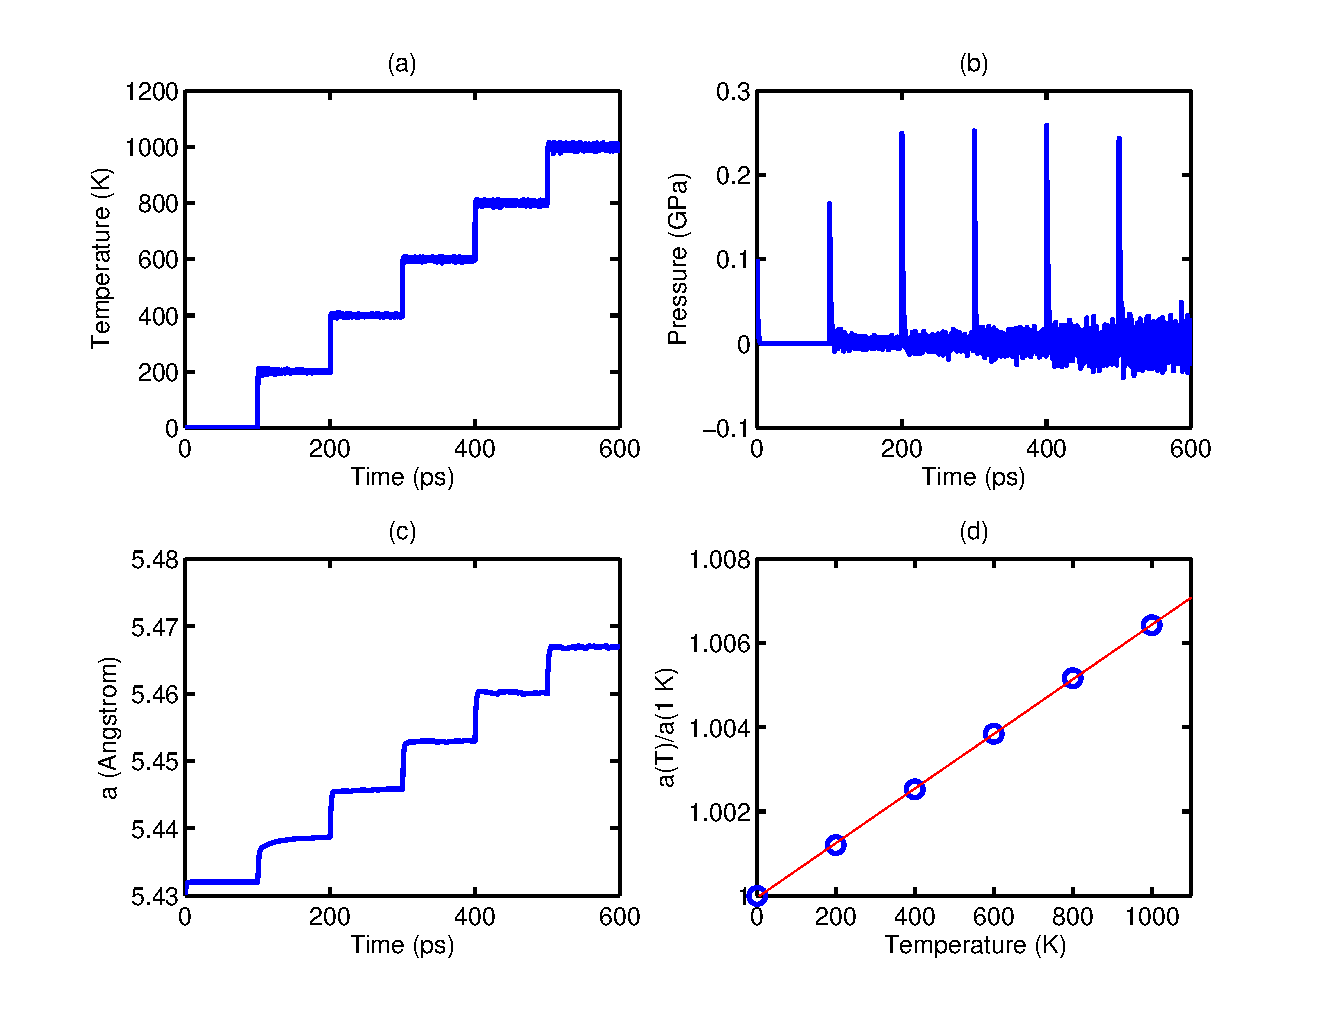
\includegraphics[width=\columnwidth]{ex1.eps}
\caption{(a) Instant temperature as a function of simulations time. (b) Instant pressure as a function of simulation time. (c) Instant lattice constant as a function of simulations time. (d) Normalized average lattice constant (over the last 50 ps in each run for a given temperature) as a function of temperature.}
\label{figure:lattice_constant}
\end{center}
\end{figure}

It takes about 4 min to run this example when a Tesla K40 card is use. The speed of the run is about $1.9 \times 10^7 ~\textmd{atom} \times \textmd{step} / \textmd{second}$.

The output file \verb"thermo.out" contains many useful data, which can be analyzed by the MATALB script \verb"plot_results.m". The results are shown in Fig. \ref{figure:lattice_constant}:
\begin{itemize}
\item (a): The temperature for each run quickly reaches the target temperature (with fluctuations).
\item (b): The pressure (averaged over the three directions) for each run quickly reaches the target pressure zero (with fluctuations).
\item (c): The lattice constant (averaged over the three directions) for each run reaches a plateau (with fluctuations) after some steps.
\item (d): We calculate the average lattice constant at each temperature by averaging the second half of the data for each run. The average lattice constants at different temperatures can be well fit by a linear function, with the thermal expansion coefficient being estimated to be $\alpha \approx 6.5\times10^{-6}$ K$^{-1}$.
\end{itemize}


\section{Phonon density of states of graphene}


In this example, we calculate the phonon density of states of graphene at 300 K
and zero pressure. The simulated cell size is about 15 nm $\times$ 15 nm (8 640 atoms).
The first few lines of the \verb"xyz.in" file are:
\begin{verbatim}
    8640 3 2.1
    1 1 0 149.649 155.52 3.35
    0 0 12 1.24708 0 0
    0 0 12 0 0.72 0
    0 0 12 0 2.16 0
    0 0 12 1.24708 2.88 0
\end{verbatim}
This is a stable structure with 3 neighbors for each atom when periodic boundary conditions are applied in the planar directions ($x$ and $y$). In the $z$ direction, free boundary conditions are used. Every atom is of type 0 and in group 0.

The \verb"run.in" file reads:
\begin{verbatim}
    #-------------------------------------------------------------------
    potential   potentials/c_tersoff_fan_2017.txt
    velocity    300

    ensemble    npt_ber 300 300 0.01 0 0 0 0.0005
    time_step   1
    dump_thermo 1000
    run         1000000

    ensemble    nve
    compute_vac 5 200 400
    run         100000

    ensemble    nve
    compute_vac 5 200 400
    run         100000

    ensemble    nve
    compute_vac 5 200 400
    run         100000

    ensemble    nve
    compute_vac 5 200 400
    run         100000

    ensemble    nve
    compute_vac 5 200 400
    run         100000
    #-------------------------------------------------------------------
\end{verbatim}

The potential model is Tersoff-1989, but some parameters are those reparameterized by Lindsay and Broido \cite{lindsay2010prb}. In the version by Lindsay and Broido, the carbon-carbon bond length at zero temperature is 1.44 \AA, which is larger than the experimental value, 1.42 \AA. Because the only relevant length parameters in the Tersoff-1989 potential are $\lambda$ and $\mu$ in the repulsive and attractive functions, we can simply correct the bond length by a proper scaling of these two parameters. All the other parameters are not affected by this scaling.

\begin{figure}[ht]
\begin{center}
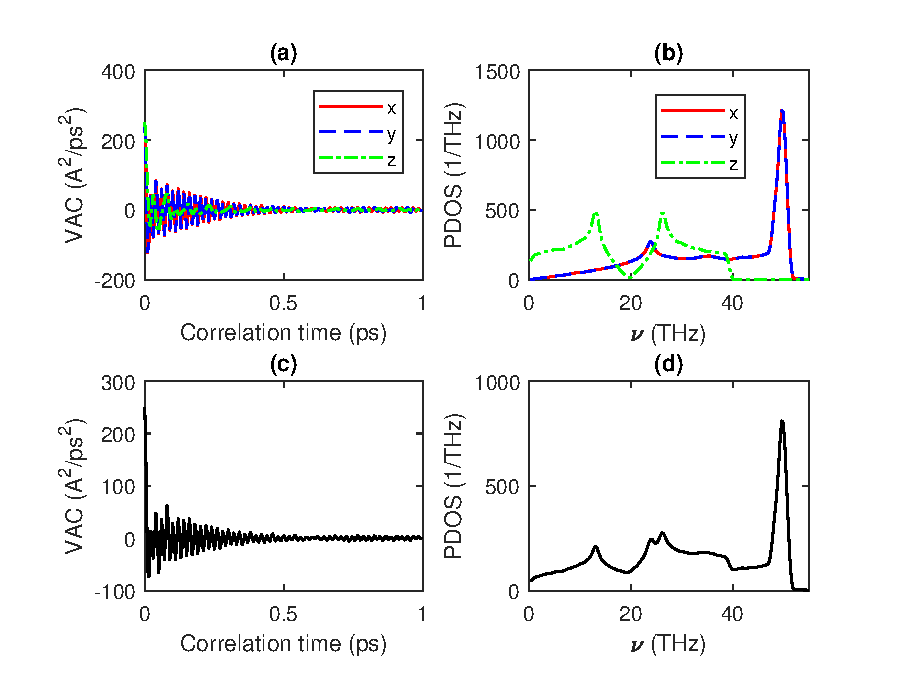
\includegraphics[width=\columnwidth]{ex2.eps}
\caption{(a) VAC as a function of correlation time for the separate directions.
(b) PDOS as a function of the phonon frequency for the separate directions.
(c) VAC as a function of correlation time averaged over the separate directions.
(d) PDOS as a function of the phonon frequency average over the separate directions.}
\label{figure:graphene_vac_dos}
\end{center}
\end{figure}

There are 6 runs. The first run serves as the equilibration stage, where the $NPT$ ensemble is used. This run lasts 1 ns. The other 5 runs are identical production runs. In each production run, the $NVE$ ensemble is used. The line with \verb"compute_vac" means that velocities will be recorded every 5 steps (5 fs) and 200 VAC data (the maximum correlation time is then about 1 ps) will be calculated. The last parameter in this line is the maximum angular frequency considered, $\omega_{\rm max} = 2\pi\nu_{\rm max} =400$ THz, which is large enough for graphene. Each production run lasts 100 ps. The major reason for using multiple production runs rather a single one is that computing the VAC requires a lot of memory, which prevents using very long runs.

This simulation takes about 7 min when a Tesla K40 is used.
The speed of this simulation, being about $3.6\times 10^7 ~\textmd{atom} \times \textmd{step} / \textmd{second}$, is higher than that of the previous example because the number of neighbors for each atom is smaller here (numbers of atoms are comparable and the potential models are the same).



Figure \ref{figure:graphene_vac_dos} shows the calculated VAC and PDOS.
For 3D isotropic systems, the results along different directions are equivalent and can be averaged, but for 2D materials like graphene, it is natural to consider the in-plane part (the $x$ and $y$ directions in the simulation) and the out-of-plane part (the $z$ direction) separately. It can be seen that the two components behave very differently. We can see that the cutoff frequency for the out-of-plane component ($\sim4 0$ THz) is smaller than that for the in-plane component ($\sim 52$ THz), which means that the two components have different Debye temperatures.


\section{Thermal conductivity of graphene}


In this example, we use the Green-Kubo method to calculate the lattice thermal conductivity of graphene at 300 K and zero pressure. The \verb"xyz.in" file and the potential parameters used are the same as in the last example. Note that the thickness of the graphene sheet is set to 3.35 \AA ~according to the convention in the literature. This thickness is needed to calculate an effective 3D thermal conductivity for a 2D material.


The \verb"run.in" file for this simulation reads:
\begin{verbatim}
    #-------------------------------------------------------------------
    potential            potentials/c_tersoff_fan_2017.txt
    velocity             300

    ensemble             npt_ber 300 300 0.01 0 0 0 0.0005
    time_step            1
    dump_thermo          1000
    run                  1000000

    ensemble             nve
    compute_hac          20 50000 10
    run                  10000000
    #-------------------------------------------------------------------
\end{verbatim}

The equilibrium stage is the same as in the last example. In the production stage, we use the NVE ensemble and calculate the HAC (heat current autocorrelation) and RTC (running thermal conductivity). The sampling interval is 20, the number of correlation steps is 50000 (such that the maximum correlation time is about $10^6$ fs = 1 ns), and the HAC and RTC are averaged for every 10 data points before written out. The production time is 10 ns, which is 10 times as long as the maximum correlation time. This is a reasonable choice.


\begin{figure}[ht]
\begin{center}
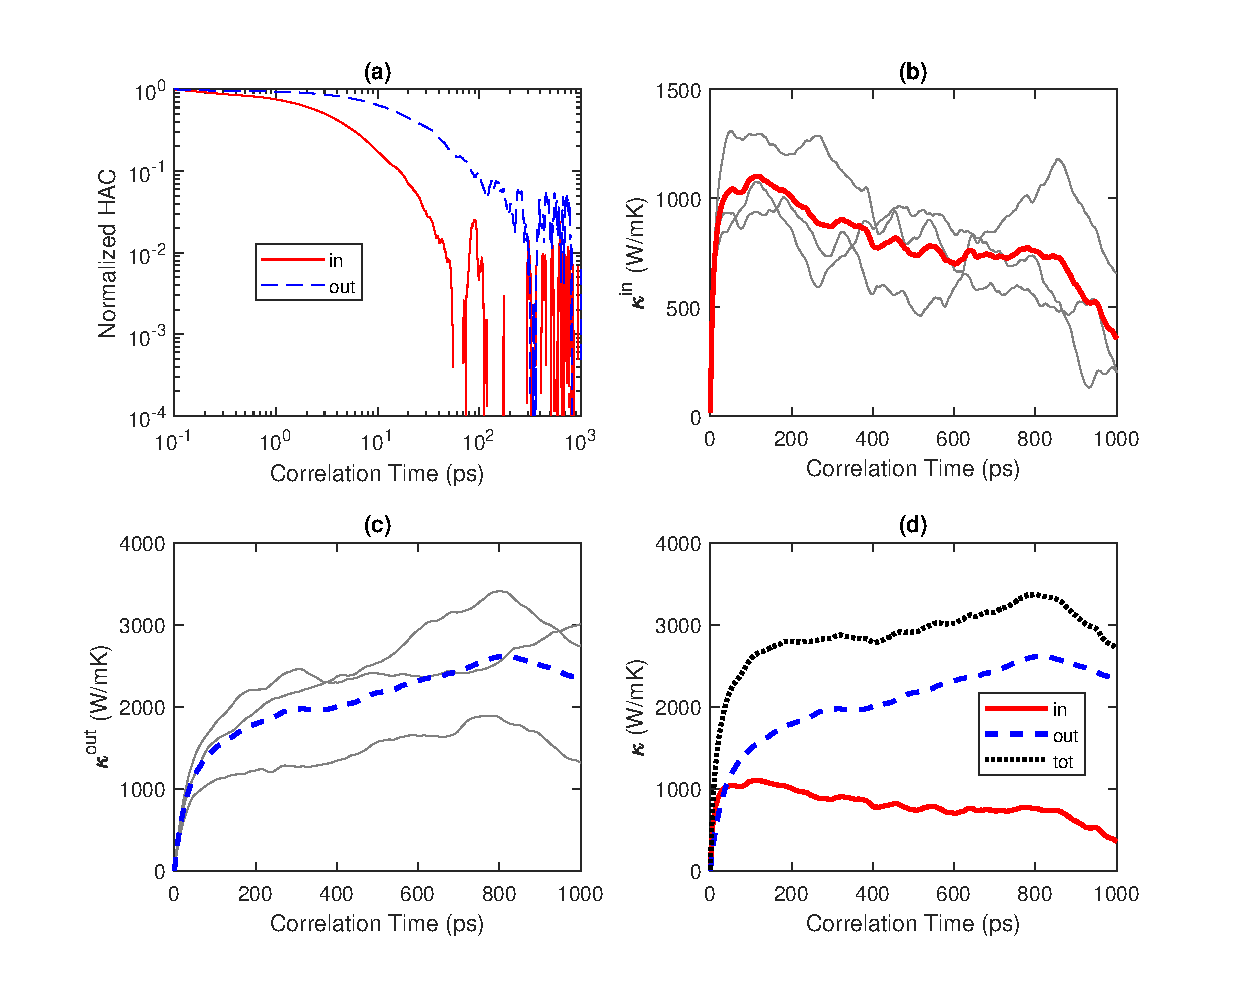
\includegraphics[width=\columnwidth]{ex3.eps}
\caption{(a) Normalized HAC as a function of correlation time for the in-plane and out-of-plane components. (b) RTC as a function of correlation time for various components. }
\label{figure:ex3}
\end{center}
\end{figure}

It takes about one hour to complete the simulation using a Tesla K40 card.
Figure shows the results from a single simulation. Note that the output file \verb"hac.out" contain decomposed HACs and RTCs as described in Ref. \cite{fan2017prb}. As the system is essentially isotropic, we can average over the two directions. The results are presented in Fig. \ref{figure:ex3}. From (a), we can see that the in-plane component and the out-of-plane component have different time scales. The latter decays much more slowly. In (b), the RTC components $\kappa^{\text{in}}$, $\kappa^{\text{out}}$, $\kappa^{\text{cross}}$, together with the RTC in the $z$ direction $\kappa_z$, are presented. It is clear that $\kappa^{\text{out}}$ converges much more slowly than $\kappa^{\text{in}}$ and to a larger magnitude. This is an accepted result stating that heat transport in suspended pristine graphene is dominated by the flexural (out-of-plane) phonons. Note that heat transport in the $z$ direction here is meaningless because free boundary conditions are applied in this direction. However, the fact that the calculated $\kappa_z$ should converged to zero can provide a validation of the results.


Accurately calculating thermal conductivity of graphene can be a very time consuming task. The results we presented are from a single simulation with a production time of 10 ns. It can been seen that the data already becomes very noisy when the correlation time is 100 ps. To obtain accurate results, one needs to do many independent simulations and do a statistical average. Much more accurate data were presented in Fig. 2 of Ref. \cite{fan2017prb}. Here are the simulation parameters used in Ref. \cite{fan2017prb} which differ from those used in this example:
\begin{itemize}
\item The simulation cell size used in Ref. \cite{fan2017prb} is larger, which is about 25 nm $\times$ 25 nm (24000 atoms).
\item The maximum correlation time used in Ref. \cite{fan2017prb} is larger, which is 10 ns.
\item The production time used in Ref. \cite{fan2017prb} for one independent simulation is larger, which is 50 ns.
\item There are 100 independent simulations in Ref. \cite{fan2017prb}, not a single one here.
\end{itemize}

Each independent simulation in Ref. \cite{fan2017prb} took about 10 GPU hours (using Tesla K40) and about 1000 GPU hours were used to obtain the results shown in Fig. 2 of Ref. \cite{fan2017prb}.


\section{Ballistic thermal conductance of graphene}

In this example, we show how to study heat transport using the NEMD method combined with the spatial and spectral decompositions as described in Ref. \cite{fan2017prb}. We aim to obtain similar results for the case of unstrained graphene as presented in Fig. 4 of Ref. \cite{fan2017prb}.

In the NEMD simulation, periodic boundary conditions are applied to the transverse direction (chosen as the zigzag direction) and fixed boundary conditions are applied to the transport direction (chosen as the armchair direction). The width of the simulated system is about 10 nm and the total length in the transport direction is about 70 nm. One major difference from the previous simulations is that here the group labels are not identically 0. We divide the system into 8 groups along the transport direction and label the groups from 1 to 8. Groups and 1 and 8 are taken as the source and sink regions, respectively. The number of atoms in groups 1 to 8 are 8000, 1600, 1600, 1600, 1600, 1600, 1600, and 8000, respectively. Some extra fixed atoms are put into group 0. Here are \textbf{two important notes} on the group label:
\begin{itemize}
\item It starts from 0.
\item In the \verb"xyz.in" file, an atom with smaller group label should appear earlier than that with a larger group label. We may remove this restriction in a future version but one should remember this rule when using the current version.
\end{itemize}

The \verb"run.in" file for this example reads:
\begin{verbatim}
    #-------------------------------------------------------------------
    potential    potentials/c_tersoff_fan_2017.txt
    velocity     300

    ensemble     nvt_ber 300 300 0.01
    fix          0
    time_step    1
    dump_thermo  1000
    run          1000000

    ensemble     heat_nhc 300 100 10 1 8
    fix          0
    compute_temp 1000
    compute_shc  2 250 100000 4 5
    run          2000000
    #-------------------------------------------------------------------
\end{verbatim}

In this simulation, we fix the lattice constant and only control the temperature in the equilibration stage. The \verb"fix 0" command is used to realize the fixed boundary conditions by fixing the atoms in group 0. In the production stage, the \verb"heat_nhc" ``ensemble'' type is used to generate the nonequilibrium heat current.  The heat source (group 1) and the heat sink (group 8) will be maintained at 310 K and 290 K, respectively. The block temperatures will be output every 1000 integration steps. The command with the keyword \verb"compute_shc" means that the nonequilibrium heat current correlation function defined in Eq. (\ref{equation:K_time}) will be computed: the sampling interval is 2, the number of correlation steps is 250, the number of steps for calculating one correlation function is 100000, and the heat current considered flows from group 4 to group 5 (the middle interface of the simulated system).


\begin{figure}[ht]
\begin{center}
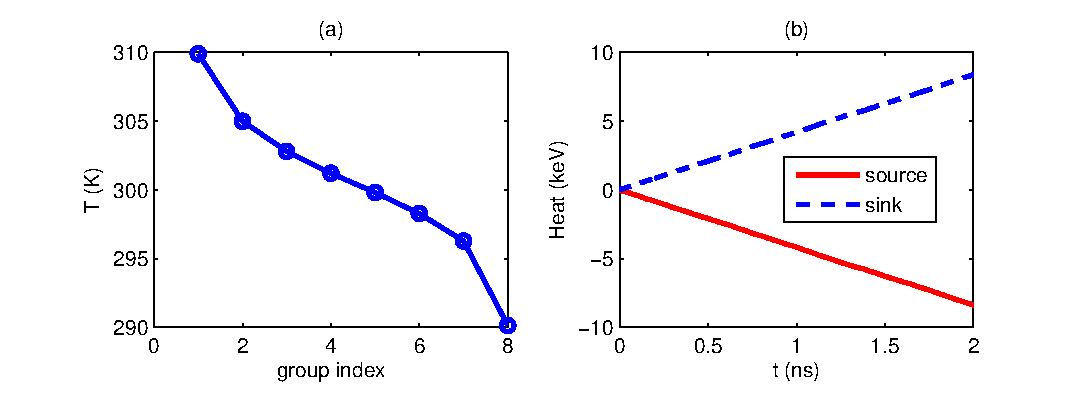
\includegraphics[width=\columnwidth]{ex4a.eps}
\caption{(a) Temperature profile in the NEMD simulation. (b) Total energy of the thermostats as a function of simulation time in the production stage. }
\label{figure:ex4a}
\end{center}
\end{figure}

This simulation takes about 40 min using a Tesla K40 card. Figure \ref{figure:ex4a} shows the results obtained from the \verb"temperature.out" file:
\begin{itemize}
\item (a): The block temperatures show a relatively smooth profile, but no clear linear region can be identified. Actually, heat transport here is ballistic and we do not expect to find a well defined temperature gradient (which is need for computing the thermal conductivity). What is important is that a well defined temperature difference (20 K), which is needed for computing the ballistic thermal conductance, can be established.
\item (b): A steady energy exchange between the system and the thermostats in the source and sink regions has been well established. The nonequilibrium heat current can be estimated to be about $Q=4.2$ eV/ps. Then a ballistic conductance of about $G=10.2$ GW m$^{-2}$ K$^{-1}$ can be obtained. This classical value overestimates the correct one and we will add discussion about quantum corrections after some of our submitted manuscripts get published.
\end{itemize}


\begin{figure}[h]
\begin{center}
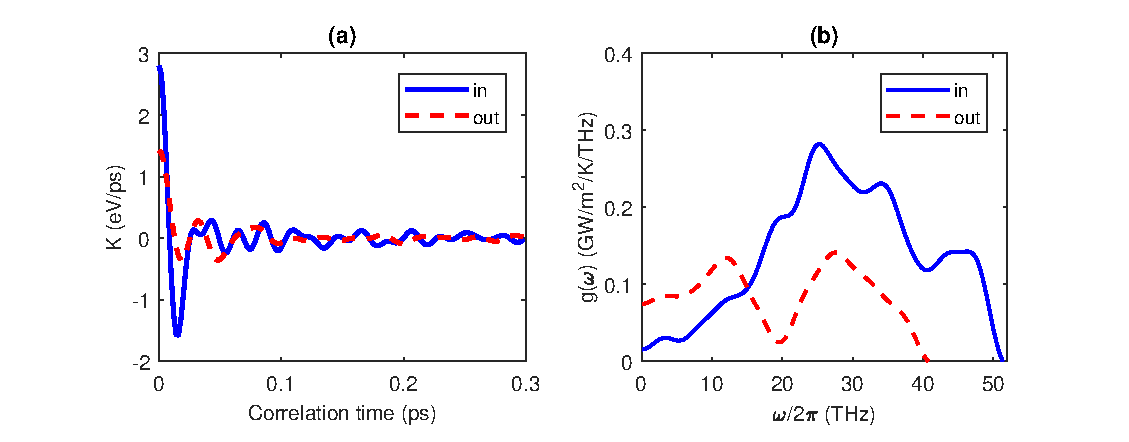
\includegraphics[width=\columnwidth]{ex4b.eps}
\caption{(a) The nonequilibrium heat current autocorrelation function as define in Eq. (\ref{equation:K_time}) as a function of correlation time. (b) The spectrally decomposed ballistic conductance as a function of phonon frequency. }
\label{figure:ex4b}
\end{center}
\end{figure}


The \verb"shc.out" file contains data for the nonequilibrium heat current autocorrelation function $K(t)$ as define in Eq. (\ref{equation:K_time}). Also, the in-out decompositions introduced in Ref. \cite{fan2017prb} is considered. The calculated $K(t)$ and the spectrally decomposed conductance $g(\omega)$ for the in-plane and the out-of-plane components are shown in Fig. \ref{figure:ex4b}. One can see that they are similar to the velocity autocorrelation and the phonon density of states discussed in a previous example. This is reasonable because the ballistic conductance is proportional to the product of the phonon density of states and the group velocity.

One can check the consistency of the results at least in the following two ways:
\begin{itemize}
\item When steady state is achieved, the correlation function $K(t)$ evaluated at zero correlation time should be consistent with the heat current calculated from the energy exchange rate between the system and the thermostats. That is, $K(0)=Q$.
\item The total thermal conductance $G$ should equal the integration of the spectral conductance. That is, $G = \int_0^{\infty} \frac{d\omega}{2\pi} g(\omega)$.
\end{itemize}
One should always make sure that the obtained data pass these tests approximately.

\bibliographystyle{plain}
\bibliography{refs}


\end{document}










